\documentclass[a4paper,12pt]{article}
\usepackage[T1]{fontenc}
\usepackage{parskip} % Removes paragraph indentation, adds vertical space between paragraphs
\usepackage{
    abraces, algorithm, algpseudocode, amsfonts, amsmath, amssymb, amsthm, bm, booktabs, enumitem, graphicx, mathtools, subcaption
}
\usepackage{natbib}
\usepackage{newtxtext,newtxmath} % modern, Times-like + proper math. Or \usepackage{lmodern}
\usepackage{newtxtt} % monospaced font
% \usepackage{zi4} % provides the Inconsolata monospaced font, but in a LaTeX-ready form
\usepackage[raggedright]{titlesec} % in case for long titles
\usepackage[breaklinks]{hyperref} % allow breaklines for references
\usepackage{cleveref} % load after hyperref package
\usepackage{minted} % for pretty code appendix
\usepackage[a4paper,left=3cm,right=3cm,top=3cm,bottom=3cm]{geometry}
\raggedbottom % don't force equal height pages. Or \flushbottom to make make pages equal height
\allowdisplaybreaks % allow page breaks inside equations 
\graphicspath{{./imgs/}{../benchmark/}{../figs/}}

\newtheorem{theorem}{Theorem}[section]
\newtheorem{definition}{Definition}[section]
\newtheorem{remark}{Remark}[section]
\newtheorem{lemma}{Lemma}[section]
\newtheorem{corollary}{Corollary}[section]
\newtheorem{prop}{Proposition}[section]

\DeclareMathOperator{\Arg}{Arg} % Branch argument of complex numbers
\DeclareMathOperator{\Var}{Var} % variance
\DeclareMathOperator{\Cov}{Cov} % covariance
\DeclareMathOperator{\corr}{corr} % correlation
\DeclareMathOperator{\Int}{Int} % interior
\DeclareMathOperator{\Ext}{Ext} % exterior
\DeclareMathOperator{\Res}{Res} % residule
\DeclareMathOperator{\tr}{tr} % trace
\DeclareMathOperator*{\argmax}{arg\,max} % argmax
\DeclareMathOperator*{\argmin}{arg\,min} % argmin
\DeclarePairedDelimiter\abs{\lvert}{\rvert} % absolute value
\DeclarePairedDelimiter\norm{\lVert}{\rVert} % norm

% Swap the definition of \abs* and \norm*, so that \abs
% and \norm resizes the size of the brackets, and the
% starred version does not.
\makeatletter
\let\oldabs\abs
\def\abs{\@ifstar{\oldabs}{\oldabs*}}
%
\let\oldnorm\norm
\def\norm{\@ifstar{\oldnorm}{\oldnorm*}}


\begin{document}
\pagenumbering{gobble} % Turn off page numbering until first section.

% Title page
\begin{titlepage}
\begin{center}
\vspace{1cm}
\textsf{\Huge{University of Oxford \\}}
\vspace{1cm}
\begin{figure}[htb]
\centering

\includegraphics[scale=.8]{stats_logo_RGB.jpg}
\end{figure}
\vspace{2.0cm}
\Huge{Score-Based Diffusion Models for Protein Backbone Generation\\}
\vspace{2.0cm}
\large{ by \\[14pt] Yuanhao Jiang \\[8pt] Wolfson College} \\
\vspace{2.2cm}
\large{A dissertation submitted in partial fulfilment of the degree of Master of Science in Statistical Science.
} \\
\vspace{.5cm}
\large{\emph{Department of Statistics, 24--29 St Giles, \\Oxford, OX1 3LB}} \\
\vspace{1.0cm}
\large{September 2025} \\
\end{center}
\end{titlepage}
\clearpage

This is my own work (except where otherwise indicated)
\vspace{2.5in}

\begin{center}
Candidate: Yuanhao Jiang\\
\vspace{1.0in}
Signed:.................................\\
\vspace{1.0in}
Date:...................................
\end{center}
\clearpage
\begin{abstract}

The abstract should go here.

\end{abstract}
\clearpage
\vspace*{2in}
\begin{center}
\textbf{Acknowledgements}
\end{center}

I would like to thank the following:
\clearpage

\tableofcontents
\listoffigures
\listoftables
\clearpage

\pagenumbering{arabic}

\section{Introduction}
\subsection{Background on Diffusion Models}
Diffusion models have recently emerged as one of the most powerful classes of deep generative models, achieving strong performance across a range of domains, most prominently in image generation \citep{hoDenoisingDiffusionProbabilistic2020,dhariwal2021DiffusionModelsBeat}. These models construct a forward process that gradually corrupts data with Gaussian noise, and train a neural network to approximate the reverse-time dynamics that iteratively remove noise. The resulting generative process is both probabilistically principled and empirically effective, offering advantages in sample quality and training stability compared to earlier paradigms such as variational autoencoders (VAEs) \citep{kingma2022AutoEncodingVariationalBayes} and generative adversarial networks (GANs) \citep{goodfellow2020GenerativeAdversarialNetworks}.

Score-based diffusion models \citep{song2019GenerativeModelingEstimating,songImprovedTechniquesTraining2020,song2021ScoreBasedGenerativeModeling,songMaximumLikelihoodTraining2021} extend denoising diffusion models by shifting the focus from directly learning the reverse process to estimating the score function, i.e.\ the gradient of the log-density of the noisy distribution, and naturally generalising the formulation to continuous time via stochastic differential equations (SDEs), allowing different forward noise processes and corresponding reverse-time samplers to be employed. The resulting framework is highly flexible and has been successfully applied to a wide range of domains, including image and audio generation, point cloud modelling, and molecular conformations.

\subsection{Motivation for Protein Structure Generation}
Proteins are essential macromolecules whose biological functions are determined by their three-dimensional structures. The ability to generate novel protein backbones has potential applications in biomedical science, including de novo protein design, drug discovery, and enzyme engineering. However, protein structures are subject to strict constraints: bond lengths and bond angles are restricted to narrow ranges, torsional angles follow characteristic distributions, and global folds must remain physically plausible \citep{creighton1993proteins,branden2012IntroductionProteinStructure}. These factors make the generative task significantly more challenging than in more common domains such as images or text.

Deep learning has already transformed structural biology. AlphaFold \citep{jumper2021HighlyAccurateProtein}, for example, demonstrated the power of data-driven methods for predicting native protein structures from amino acid sequences. However, the problem of generating realistic and diverse protein structures remains comparatively underexplored.

\subsection{Diffusion Models for Protein Structures}
The probabilistic formulation of score-based diffusion models makes them a natural candidate for modelling protein backbones. Unlike GANs, diffusion models provide a likelihood-based framework, and unlike VAEs, they do not impose restrictive assumptions on the latent space. Their iterative denoising dynamics also align well with the idea of progressively refining approximate structures toward physically plausible conformations.

Recent works highlight this promise. \citet{watsonNovoDesignProtein2023} introduced a diffusion-based framework for de novo design, achieving impressive results in generating novel folds and functional proteins. \citet{wuProteinStructureGeneration2024} modelled folding trajectories using diffusion, while \citet{yimDiffusionModelsProtein2024} applied diffusion models to protein-ligand docking, demonstrating the versatility of the paradigm in structural biology. These advances suggest that diffusion models can capture rich geometric and biophysical constraints in a principled way.

A key challenge lies in representation. In this work, we represent the protein backbone as a graph where nodes correspond to C\(_\alpha\) atoms and edges encode both spatial proximity and sequential adjacency. This formulation enables the use of graph neural networks (GNNs) \citep{scarselliGraphNeuralNetwork2009,gilmer2017NeuralMessagePassing} as score models, incorporating geometric features such as radial basis encodings, directional vectors, and positional embeddings. In particular, we employ Transformer-based graph convolutional layers, which extend the expressive power of message passing beyond classical GCNs \citep{kipf2017SemiSupervisedClassificationGraph}. Training such models on structural datasets allows the score function to be learned over backbone conformational space, from which new structures can be sampled by reverse diffusion.

\subsection{Structure of the Dissertation}
The remainder of this dissertation is organised as follows. \Cref{sec:SBD} introduces the theoretical framework of score-based diffusion models and their formulation via stochastic differential equations. \Cref{sec:protein-gnn} presents the graph-based representation of protein backbones and the neural architectures considered in this study. \Cref{sec:Experiments} reports experimental results on the CATH S40 dataset, including quantitative metrics and qualitative visualisations. Finally, \Cref{sec:Discussion_and_Conclusion} discusses the results, outlines limitations, and highlights directions for future work.

\clearpage

\section{Score-Based Diffusion for Generative Modelling}\label{sec:SBD}
\subsection{Background and Motivation}
Generative modelling aims to learn a distribution from which new samples can be drawn that resemble those observed in a dataset. Classical approaches include variational autoencoders (VAEs)~\citep{kingma2022AutoEncodingVariationalBayes}, which maximise a variational lower bound on the likelihood, and generative adversarial networks (GANs)~\citep{goodfellow2020GenerativeAdversarialNetworks}, which frame generation as an adversarial game. While each of these paradigms has been successful, they also suffer from characteristic drawbacks such as blurry reconstructions (VAEs) and mode collapse (GANs).

Diffusion models represent a more recent class of generative models that address many of these limitations. The central idea is deceptively simple: one defines a forward process that gradually corrupts data with noise until the signal is destroyed, and then learns a reverse process that reconstructs data from noise. By formulating the forward process as a diffusion and training a neural network to approximate the reverse dynamics, diffusion models combine the flexibility of deep networks with the probabilistic rigour of latent-variable models. 

In their original formulation, denoising diffusion probabilistic models (DDPMs)~\citep{hoDenoisingDiffusionProbabilistic2020} defined the forward process as a discrete-time Gaussian Markov chain. Subsequent work by \citet{song2021ScoreBasedGenerativeModeling} showed that diffusion models can be generalised to continuous-time stochastic differential equations (SDEs). In this framework, the key object is the score function, i.e.~the gradient of the log-density of the noisy distribution. Learning this score function allows one to simulate the reverse SDE and thereby generate new samples.

This chapter develops the theoretical foundations of score-based diffusion models in detail. We begin with the definition of the forward diffusion process, proceed to the derivation of the reverse-time dynamics, introduce score matching as the training objective, and describe practical sampling algorithms and noise schedules. Together, these elements form the mathematical basis for applying diffusion models to protein backbone generation in later chapters.

\subsection{Forward Diffusion Processes}
The first component of a diffusion generative model is the forward, or noising, process. 
This process gradually perturbs the data distribution into a tractable prior distribution, typically a standard Gaussian. The key requirement is that this transformation be both easy to sample from and analytically tractable, so that training objectives can be computed efficiently.

\subsubsection{Discrete-Time Formulation}
Denote clean data samples by \(x_0 \sim p_{\text{data}}(x)\). Denoising diffusion probabilistic models (DDPMs)~\citep{hoDenoisingDiffusionProbabilistic2020} define the forward process as a Markov chain of \(N\) steps:
\begin{align*}
    q\left(x_{1:N}\mid x_0\right)\coloneq\prod_{i=1}^{N}q\left(x_i|x_{i-1}\right),
\end{align*}
where each transition adds a small amount of Gaussian noise,
\begin{align}\label{eq:DDPM-transition-kernel}
    q\left(x_i \mid x_{i-1}\right)\coloneq\mathcal{N}\!\left(x_i ; \sqrt{1-\beta_i}\,x_{i-1}, \, \beta_i I \right),\quad i=1,...,N.
\end{align}
This produces a sequence of progressively noisier variables \(\{x_i\}_{i=1}^N\). Here, \(\{\beta_i\}_{i=1}^N\) is a variance schedule with \(\beta_i \in (0,1)\) controlling the noise injected at each step.

A key property of the Gaussian forward process is that one can sample \(x_t\) at any arbitrary time step directly from the data \(x_0\):
\begin{align}\label{eq:DDPM-solution}
    q\left(x_i \mid x_0\right) = \mathcal{N}\!\left(x_i ; \sqrt{\bar \alpha_i}\,x_0, \,(1-\bar \alpha_i) I \right),
\end{align}
where \(\alpha_i = 1 - \beta_i\) and \(\bar \alpha_i = \prod_{s=1}^i \alpha_s\). This closed form is crucial for training, as it allows drawing noisy samples \(x_t\) without explicitly simulating all intermediate steps.

\subsubsection{Continuous-Time Formulation}\label{sec:forward-SDE-continuous}
\citet{song2021ScoreBasedGenerativeModeling} generalised the discrete diffusion process to continuous time by taking the limit as \(N \to \infty\) and \(\beta_i \to 0\). In this setting, the forward process can be expressed as a stochastic differential equation (SDE) of the form
\begin{align}\label{eq:forward_sde}
    dx = f(x,t)\,dt + g(t)\,dw,
\end{align}
where \(w\) is the Brownian motion, \(f(x,t)\) is a drift term, and \(g(t)\) controls the diffusion magnitude. The SDE produces a trajectory of continuously noisier variables \(\{x(t)\}_{t \in [0,T]}\).

For DDPM Gaussian transition kernel \cref{eq:DDPM-transition-kernel}, the chain is equivalent to
\begin{align*}
    x_{i}=\sqrt{1-\beta_{i}}\,x_{i-1}+\sqrt{\beta_{i}}\,z_{i-1},\quad i=1,...,N,
\end{align*}
where \(z_{i-1}\sim \mathcal{N}\!\left(0,I\right)\). Define functions \(\beta\!\left(\frac{i}{N}\right)\coloneq N\beta_i\), \(x\!\left(\frac{i}{N}\right)=x_i\) and \(z\left(\frac{i}{N}\right)=z_i\), stepsize \(\Delta t\coloneq 1/N\) and finally reparameterise the time as \(t=i\Delta t\in\left\{0,\Delta t,...,N\Delta t=1\right\}\), we have
\begin{align*}
    x\!\left(t\right)
    &=\sqrt{1-\beta\!\left(t\right)\Delta t}\,x\!\left(t-\Delta t\right)+\sqrt{\beta\!\left(t\right)\Delta t}\,z\left(t-\Delta t\right)\\
    &\overset{\Delta t\ll 1}{\approx}\left(1-\frac{1}{2}\beta\!\left(t\right)\Delta t\right)x\!\left(t-\Delta t\right)+\sqrt{\beta\!\left(t\right)\Delta t}\,z\left(t-\Delta t\right),
\end{align*}
that is
\begin{align*}
    x\!\left(t\right)-x\!\left(t-\Delta t\right)=-\frac{1}{2}\beta\!\left(t\right)\Delta t x\!\left(t-\Delta t\right)+\sqrt{\beta\!\left(t\right)\Delta t}\,z\left(t-\Delta t\right).
\end{align*}
In the limit of \(\Delta t\to0\), the above equation converges to
\begin{align}\label{eq:VPSDE}
    dx=-\frac{1}{2}\beta\!\left(t\right)xdt+\sqrt{\beta\!\left(t\right)}dw.
\end{align}
\Cref{eq:VPSDE} is refered to as the Variance-preserving (VP) SDE, where \(\beta(t)\) is the noise schedule (e.g.~linear, cosine). Just like the discrete case of DDPM, VP SDE has a closed form solution. Define
\begin{align*}
    u\left(x\!\left(t\right),t\right)=\exp\left(\frac{1}{2}\int_0^t\beta\!\left(s\right)ds\right)x\!\left(t\right).
\end{align*}
Then by It\^{o}'s chain rule, \(y\left(t\right)\coloneq u\left(x\!\left(t\right),t\right)\) has the SDE
\begin{align*}
    dy
    &=\frac{1}{2}\beta\!\left(t\right)\exp\left(\frac{1}{2}\int_0^t\beta\!\left(s\right)ds\right)x\!\left(t\right)dt+\exp\left(\frac{1}{2}\int_0^t\beta\!\left(s\right)ds\right)dx\\
    &=\exp\left(\frac{1}{2}\int_0^t\beta\!\left(s\right)ds\right)\left(\frac{1}{2}\beta\!\left(t\right)x\!\left(t\right)dt-\frac{1}{2}\beta\!\left(t\right)x\!\left(t\right)dt+\sqrt{\beta\!\left(t\right)}dw\right)\\
    &=\exp\left(\frac{1}{2}\int_0^t\beta\!\left(s\right)ds\right)\sqrt{\beta\!\left(t\right)}dw.
\end{align*}
Integrate from \(0\) to \(t\) yields
\begin{align*}
    y\!\left(t\right)=y\!\left(0\right)+\int_0^t\exp\left(\frac{1}{2}\int_0^s\beta\!\left(u\right)du\right)\sqrt{\beta\!\left(s\right)}dw_s.
\end{align*}
Now undo the change of variables we have
\begin{align*}
    x\!\left(t\right)
    &=\left[\exp\left(\frac{1}{2}\int_0^t\beta\!\left(s\right)ds\right)\right]^{-1}y\!\left(t\right)\\
    &=\exp\left(-\frac{1}{2}\int_0^t\beta\!\left(s\right)ds\right)x\!\left(0\right)+\int_0^t\exp\left(-\frac{1}{2}\int_s^t\beta\!\left(u\right)du\right)\sqrt{\beta\!\left(s\right)}dw_s.
\end{align*}
The initial condition \(x\!\left(0\right)=x_0\) is a sample from dataset, i.e.,~a constant, so the posterior of perturbation (or the prior of the reverse sampling) is a Gaussian distribution with mean
\begin{align}\label{eq:VPSDE-solution-mean}
    \mathbb{E}\left[x\!\left(t\right)\mid x\!\left(0\right)=x_0\right]=\exp\left(-\frac{1}{2}\int_0^t\beta\!\left(s\right)ds\right)x_0
\end{align}
and variance
\begin{align}
    \nonumber
    \Var\left[x\!\left(t\right)\mid x\!\left(0\right)=x_0\right]
    &=\int_0^t\exp\left(-\int_s^t\beta\!\left(u\right)du\right)\beta\!\left(s\right)ds I\\
    \label{eq:VPSDE-solution-variance}
    &=\left(1-\exp\left(-\int_0^t\beta\!\left(s\right)ds\right)\right)I
\end{align}
that is
\begin{align}\label{eq:VPSDE-solution}
    p\!\left(x_t|x_0\right)=\mathcal{N}\left(x_t:\:x_0e^{-\frac{1}{2}\int_0^t\beta(s)ds},\left(1-e^{-\int_0^t\beta(s)ds}\right)I\right).
\end{align}
Obviously the variance is always bounded, hence the name variance-preserving. This continuous formulation provides a flexible mathematical foundation that unifies discrete DDPMs with stochastic differential equations, and it allows the use of stochastic calculus tools to analyse and manipulate diffusion models. In particular, it enables the derivation of the reverse-time SDE, which defines the generative process and will be introduced in the next section.

Other choices of \(f\) and \(g\) in \cref{eq:forward_sde} yield different diffusion processes, \citet{song2021ScoreBasedGenerativeModeling} shown three categories,
\begin{itemize}
    \item \textbf{Variance-preserving (VP) SDE}: maintains the marginal variance of \(x_t\) at one throughout the process.  
    \item \textbf{Variance-exploding (VE) SDE}: variance grows unbounded as \(t \to T\), pushing the distribution to white noise.  
    \item \textbf{Sub-variance-preserving (sub-VP) SDE}: an interpolation between VP and VE.  
\end{itemize}
We will focus on VP SDE in this dissertation.

\subsection{Reverse-Time Diffusion Processes}
The forward diffusion process, whether in discrete or continuous form, progressively perturbs data until its distribution approaches a simple prior such as an isotropic Gaussian. To perform generative modelling, we require a process that inverts this corruption: starting from noise and evolving back toward the data distribution. This is formalised through the theory of time-reversal for diffusion processes.

\subsubsection{Discrete-Time Reverse Process}
In the discrete DDPM formulation~\cite{hoDenoisingDiffusionProbabilistic2020}, the generative model is defined as a reverse Markov chain
\begin{align*}
    p_\theta\left(x_{0:N}\right) \coloneq p(x_N) \prod_{i=1}^{N} p_\theta(x_{i-1} \mid x_i),
\end{align*}
with \(p(x_N) = \mathcal{N}(x_N;0,I)\) as the prior. The reverse conditionals are modelled as Gaussians
\begin{align*}
    p_\theta\left(x_{i-1} \mid x_t\right) \coloneq \mathcal{N}\!\big(x_{i-1}; \mu_\theta(x_i,i), \Sigma_\theta(x_i,i)\big),
\end{align*}
where \(\mu_\theta\) and \(\Sigma_\theta\) are learned using a neural network with parameter \(\theta\). Training then consists of minimising the Kullback-Leibler divergence between the true posterior \(q(x_{i-1} \mid x_i, x_0)\) and the model distribution \(p_\theta(x_{i-1} \mid x_i)\).

\subsubsection{Continuous-Time Reverse SDE}
In the continuous-time setting, \citet{andersonReversetimeDiffusionEquation1982} established that the time reversal of an It\^{o} SDE \eqref{eq:forward_sde}
is itself an SDE with modified drift term,
\begin{align}\label{eq:reverse_sde}
    dx = \left[f(x,t) - g^2(t) \nabla_x \log p_t(x)\right]\,dt + g(t)\,d\bar w,
\end{align}
where \(\bar w\) is the Brownian motion running backward in time, \(\nabla_x \log p_t(x)\) is the score function at time \(t\), that is, the gradient of the log-density of the perturbed, marginal, data distribution \(p_t\left(x\right)\). This equation defines the reverse-time SDE. It depends explicitly on the score function \(\nabla_x \log p_t(x)\) of the forward process marginal distribution \(p_t(x)\).

For VP SDE \cref{eq:VPSDE}, the reverse-time SDE is given by
\begin{align*}
    dx=\left[-\frac{1}{2}\beta\!\left(t\right)x-\beta\!\left(t\right)\nabla_x \log p_t(x)\right]dt+\sqrt{\beta\!\left(t\right)}d\bar w.
\end{align*}
Though it has no closed form sulution, if one can estimate the score function accurately for all times \(t\), it becomes possible to simulate the reverse SDE and generate samples from the data distribution.

This result provides the key insight underlying score-based diffusion: generative modelling reduces to score estimation. 
Rather than directly modelling likelihoods or sampling distributions, we train a neural network \(s_\theta(x,t)\) to approximate the score \(\nabla_x \log p_t(x)\). The network is then used to guide the drift of the reverse SDE, producing realistic samples when integrated from Gaussian noise at \(t = 1\) back to \(t = 0\).

\subsection{Score Matching and Training Objective}
The reverse-time SDE depends on the score function \(\nabla_x \log p_t(x)\), which is generally intractable. Thus, the central learning problem in score-based diffusion is to approximate this score with a neural network \(s_\theta(x,t)\), called time dependent score network (TDSN) \citep{song2021ScoreBasedGenerativeModeling}. Training requires a loss function that encourages \(s_\theta\) to match the true score across noise levels.

\subsubsection{Score Matching and Denoising Score Matching}\label{sec:SM-and-DSM}
For each time \(t\), the score function of \(x_t\) can be trained via minimising the Fisher divergence
\begin{align*}
    \mathbb{E}_{p\left(x_t\right)}\left[\norm{\nabla_{x_t}\log p\left(x_t\right)-s_{\theta}\left(x_t, t\right)}_2^2\right].
\end{align*}
The unknown term \(\nabla_{x_t}\log p\left(x_t\right)\) (true score) can be eliminated with the score matching objective \cite{hyvarinenEstimationNonNormalizedStatistical2005}
\begin{align*}
    J^{\text{SM}}_t(\theta)=\mathbb{E}_{p\left(x_t\right)}\left[\norm{\tr\left(\nabla_{x_t}s_{\theta}\left(x_t,t\right)\right)-\frac{1}{2}\norm{s_{\theta}(x_t,t)}_2^2}_2^2\right].
\end{align*}
Note that the term \(\tr\left(\nabla_{x_t}s_{\theta}\left(x_t,t\right)\right)\) can be computationally intensive. \citet{vincentConnectionScoreMatching2011} showed that training a denoising autoencoder to reconstruct clean data from corrupted observations is equivalent to score matching under certain conditions. This connection underpins the training of diffusion models: the neural network is trained to denoise \(x_t\) into \(x_0\), thereby learning the score function implicitly. Hence, in the case of VP SDE, since we have the analytic form of the posterior, \cref{eq:VPSDE-solution}, the denoising score matching objective is given by
\begin{align*}
    J^{\text{DSM}}_t
    &=\mathbb{E}_{x_0\sim p_{\text{data}}\left(x_0\right)}\mathbb{E}_{x_t\sim p\left(x_t|x_0\right)}\left[\norm{s_{\theta}\left(x_t,t\right)-\nabla_{x_t}\log p\left(x_t|x_0\right)}_2^2\right]\\
    &=\mathbb{E}_{x_0\sim p_{\text{data}}\left(x_0\right)}\mathbb{E}_{x_t\sim p\left(x_t|x_0\right)}\left[\norm{s_{\theta}\left(x_t,t\right)+\frac{x_t-\mu_{t}}{\sigma_t^2}}_2^2\right]
\end{align*}
where \(\mu_t\) and \(\sigma_t^2\) are given by \cref{eq:VPSDE-solution-mean,eq:VPSDE-solution-variance}, respectively.

The denoising score matching objective \(J^{\text{DSM}}_t\) is for a specific time \(t\). To train the score model across all time \(t\in\left[0,1\right]\) in one go, the overall objective is given by a weighted sum (or average) \citep{song2021ScoreBasedGenerativeModeling}
\begin{align}\label{eq:DSM}
    J^{\text{DSM}}=\mathbb{E}_{t\sim\mathcal{U}(0,1)}\left[\lambda\!\left(t\right)J^{\text{DSM}}_t\right],
\end{align}
where \(\lambda\!\left(t\right)\) is a positive weighting function.

The learning problem for score-based diffusion therefore reduces to denoising score matching: the neural network \(s_\theta(x,t)\) is trained to approximate \(\nabla_x \log p_t(x)\) across different noise levels. Once trained, this network can be used to drive the reverse SDE, enabling generation of new samples from Gaussian noise.

\subsection{Sampling Procedures}
Once the score network \(s_\theta(x,t)\) has been trained, new samples can be generated by simulating the reverse diffusion process. This requires integrating the reverse-time SDE \eqref{eq:reverse_sde} starting from Gaussian noise \(x\!\left(t=1\right) \sim \mathcal{N}(0,I)\) and evolving toward \(t=0\).

\subsubsection{Reverse SDE Sampling via Euler-Maruyama Method}
The simplest approach is to discretise the reverse SDE using the Euler-Maruyama method. For a decreasing sequence of time steps \(\{t_i\}_{i=0}^N\) with \(t_N = 1\) and \(t_0 = 0\), the update rule is
\begin{align}\label{eq:Euler-Maruyama-reverse-SDE}
    x_{t_{i-1}} = x_{t_i} + \left[f(x_{t_i},t_i) - g(t_i)^2 s_\theta(x_{t_i},t_i)\right]\Delta t + g(t_i)\sqrt{\Delta t}\,z_i,
\end{align}
where \(z_i \sim \mathcal{N}(0,I)\) and \(\Delta t = t_{i-1} - t_i\). This procedure generates approximate samples from the data distribution. While straightforward, its quality depends heavily on the number of discretisation steps: smaller steps yield higher fidelity at the cost of computational time.

\subsubsection{Predictor-Corrector Sampling}\label{sec:PC-sampling}
The Predictor-Corrector sampler was proposed by \citet{song2021ScoreBasedGenerativeModeling} as an improved sampling method. It is based on combining two components:
\begin{enumerate}
    \item \textbf{Predictor step:} one update using the reverse SDE (e.g., via Euler-Maruyama method, \cref{eq:Euler-Maruyama-reverse-SDE}), advancing the trajectory toward lower noise levels.
    \item \textbf{Corrector step:} one or more steps of stochastic refinement, implemented as Langevin Monte Carlo:
        \begin{align*}
            x \leftarrow x + \epsilon\, s_\theta(x,t) + \sqrt{2\epsilon}\,z, \quad z \sim \mathcal{N}(0,I),
        \end{align*}
        where \(\epsilon\) is a step size. This step locally improves sample quality by pushing the state toward regions of higher density according to the trained score network.
\end{enumerate}
By alternating predictor and corrector steps, the algorithm achieves a better trade-off between quality and efficiency than pure reverse SDE sampling. 
In practice, only a few corrector iterations per time step are needed to significantly improve sample fidelity.

In this dissertation, we use predictor-corrector sampling as our default procedure.

\subsection{Noise Schedules}
The design of the noise schedule plays a central role in the performance of score-based diffusion models. 
The schedule determines how the variance of the forward diffusion process evolves over time, which directly influences both training stability and the quality of generated samples.

\subsubsection{Linear Schedules}
In the original DDPM formulation \citep{hoDenoisingDiffusionProbabilistic2020}, the variance schedule \(\{\beta_i\}_{i=1}^N\) was chosen to increase linearly from a small value to a larger one over \(N\) steps. Equivalently, in the continuous SDE formulation \citep{song2021ScoreBasedGenerativeModeling}, this corresponds to a linear growth of the noise rate
\begin{align*}
    \beta\!\left(t\right)=\beta_0+\left(\beta_1-\beta_0\right)t.
\end{align*}
While simple, this schedule can be suboptimal: early time steps may inject too little noise, leading to poor coverage of high-noise regions during training, while later steps may over-noise the data, resulting in wasted computation.

\subsubsection{Cosine Variance-Preserving Schedule}\label{sec:Cos-schedule}
\citet{nicholImprovedDenoisingDiffusion2021} proposed a cosine schedule for the noising process in DDPM, which has since become widely adopted \citep{dhariwal2021DiffusionModelsBeat,saharia2022PhotorealisticTexttoImageDiffusion,watsonNovoDesignProtein2023}. The proposed cosine schedule corresponds to using
\begin{align*}
    \bar \alpha_i = \frac{\cos^2\!\left(\frac{\pi}{2}\cdot\frac{i/N+s}{1+s}\right)}{\cos^2\!\left(\frac{\pi}{2}\frac{s}{1+s}\right)}
\end{align*}
in \cref{eq:DDPM-solution} for noising process, where \(s\) is a very small offset (typically \(10^{-4}\)) to prevent singularities, that is (ignoring the denominator in \(\bar{\alpha}_i\) as it is nearly \(1\) for small \(s\)),
\begin{align*}
    x_i=\sqrt{\bar\alpha_i}\,x_0+\sqrt{1-\bar\alpha_i}\,z_i,\quad\bar\alpha_i\approx\cos^2\!\left(\frac{\pi}{2}\cdot\frac{i/N+s}{1+s}\right),\quad z_i\sim\mathcal{N}\!\left(0, I\right).
\end{align*}
This is a DDPM perturbation scheme. To generalise to continuous time, we do exactly the same as in \cref{sec:forward-SDE-continuous}: define function \(\bar{\alpha}\!\left(\frac{i}{N}\right)\coloneq\bar\alpha_i\), stepsize \(\Delta t\coloneq 1/N\) and time as \(t=i\Delta t\in\left\{0,\Delta t,...,N\Delta t=1\right\}\). This yields the continuous time schedule
\begin{align*}
    x\!\left(t\right)=\sqrt{\bar\alpha\!\left(t\right)}\,x\!\left(0\right)+\sqrt{1-\bar\alpha\!\left(t\right)}\,z\!\left(t\right),\quad\bar\alpha\!\left(t\right)=\cos^2\left(\frac{\pi}{2}\cdot\frac{t+s}{1+s}\right),\quad z\!\left(t\right)\sim\mathcal{N}\!\left(0, I\right).
\end{align*}
Match with previous derivation, \cref{eq:VPSDE-solution}, we are left to solve
\begin{align*}
    \bar\alpha\!\left(t\right)=e^{-\int_0^t\beta(s)ds}.
\end{align*}
It follows that
\begin{align}
    \nonumber
    \beta(t)
    &=-\frac{d}{dt}\log\cos^2\left(\frac{\pi}{2}\cdot\frac{t+s}{1+s}\right)\\
    \nonumber
    &=-\frac{1}{\cos^2\left(\frac{\pi}{2}\cdot\frac{t+s}{1+s}\right)}\left[2\cos\left(\frac{\pi}{2}\cdot\frac{t+s}{1+s}\right)\right]\left[-\sin\left(\frac{\pi}{2}\cdot\frac{t+s}{1+s}\right)\right]\frac{d}{dt}\left(\frac{\pi}{2}\cdot\frac{t+s}{1+s}\right)\\
    \label{eq:cosine-beta}
    &=\frac{\pi}{1+s}\tan\left(\frac{\pi}{2}\cdot\frac{t+s}{1+s}\right).
\end{align}
Instead of linear growth, the cosine schedule ensures a smoother increase in noise variance, the noising strength changes much slower near \(i=1\) and \(i=N\), as illustrated by \cref{fig:schedule-linear-vs-cosine}. This schedule maintains higher signal levels for longer, enabling the score network to learn more effectively across a wider range of noise intensities.

\begin{figure}[htbp]
    \centering
    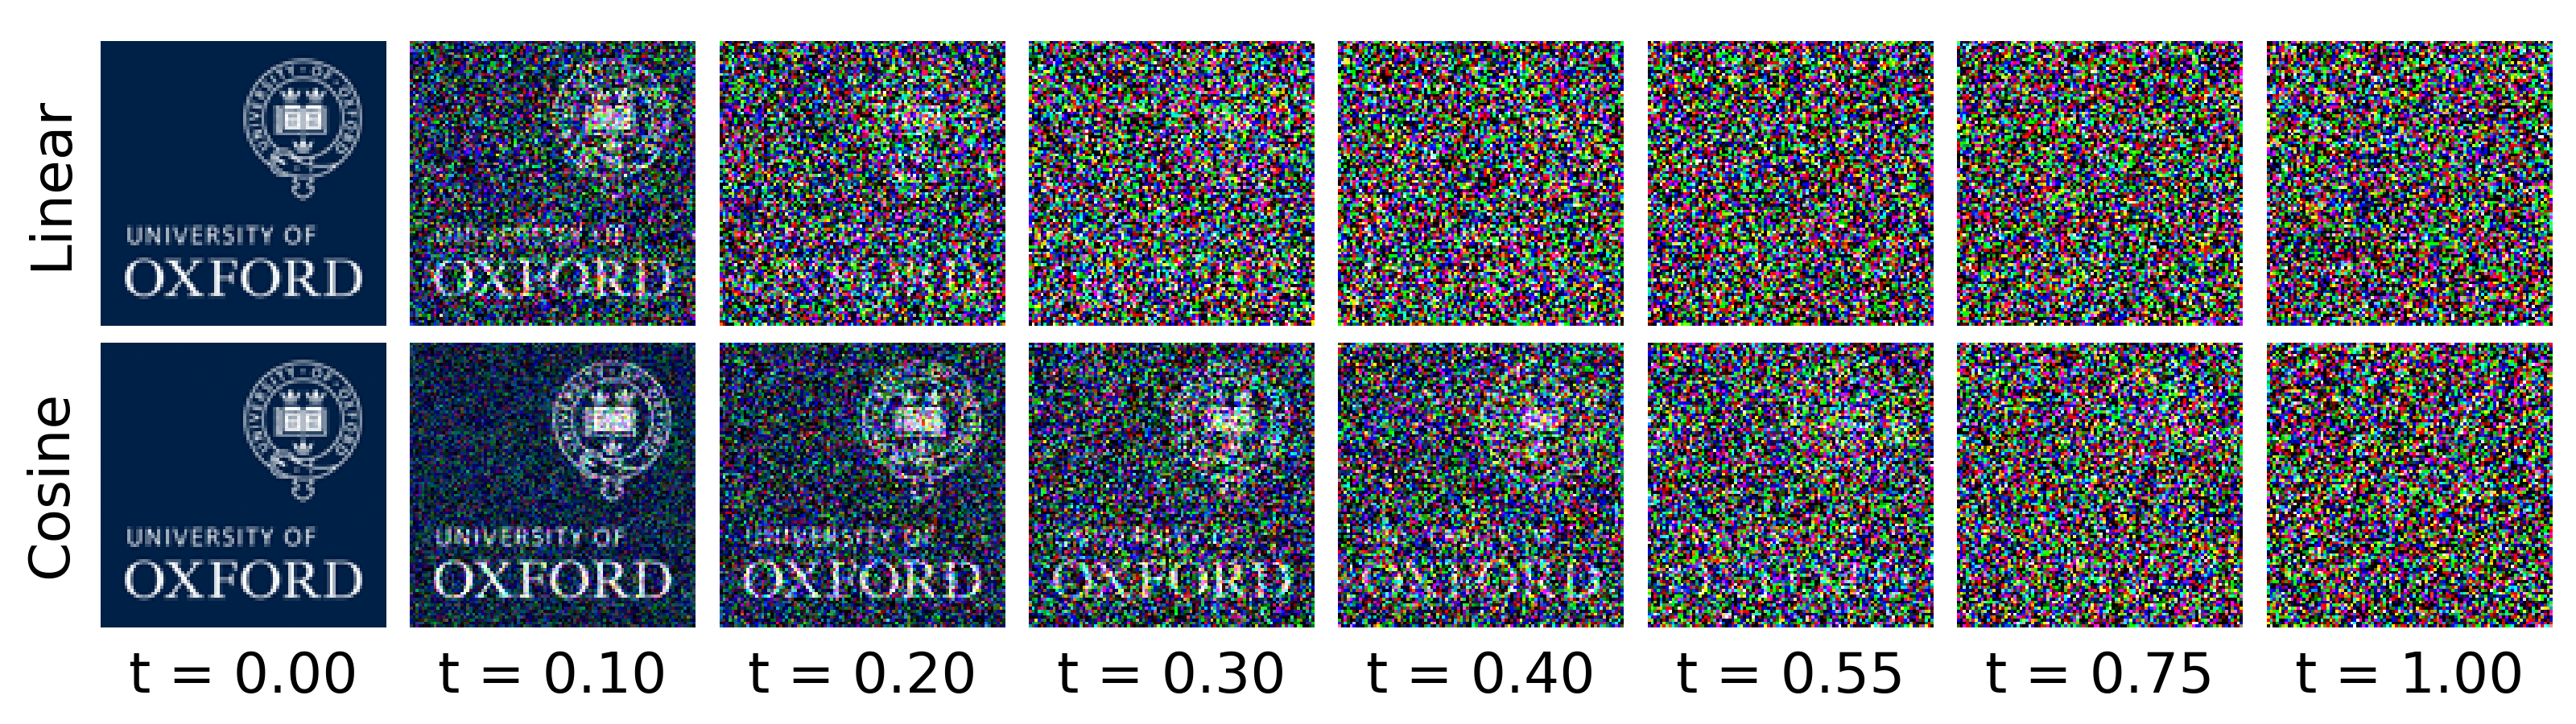
\includegraphics[width=\linewidth]{linear_vs_cosine.png}
    \caption{Linear schedule vs. cosine schedule.}
    \label{fig:schedule-linear-vs-cosine}
\end{figure}

Empirically, the cosine schedule improves sample quality and accelerates convergence compared to linear schedules. It balances the trade-off between injecting sufficient noise for diversity and preserving enough signal for stable training. Moreover, because it avoids excessively noisy late stages, fewer discretisation steps are needed during sampling, reducing computational cost.

In this dissertation, we adopt this cosine schedule as the forward diffusion process. This choice is motivated by its demonstrated effectiveness in image and structural generative tasks \citep{dhariwal2021DiffusionModelsBeat,saharia2022PhotorealisticTexttoImageDiffusion,watsonNovoDesignProtein2023}, and by its compatibility with the variance-preserving SDE formulation used in our score model, \cref{eq:cosine-beta}. All experiments in later chapters therefore use the cosine schedule as the default setting.

\subsection{Summary}
This chapter has established the theoretical foundations of score-based diffusion models, which form the core generative framework employed in this dissertation. We began by introducing the forward diffusion process, first in its discrete DDPM formulation and then in its continuous-time generalisation as a stochastic differential equation. We then derived the reverse-time SDE, showing that generative modelling reduces to the problem of score estimation. This led naturally to the denoising score matching objective, which enables training a neural network to approximate the score function across all noise levels. Finally, we discussed practical sampling algorithms, including reverse SDE integration and predictor-corrector methods, and examined the role of noise schedules, with particular emphasis on the cosine variance-preserving schedule adopted in this work.

Together, these elements provide a principled probabilistic framework for deep generative modelling. Unlike GANs or VAEs, score-based diffusion models avoid common issues such as mode collapse or restrictive latent assumptions, while offering strong theoretical guarantees and flexible sampling procedures. The remainder of this dissertation builds upon these foundations to adapt score-based diffusion to the setting of protein backbone generation, where structural constraints and geometric representations introduce unique modelling challenges.

\clearpage

\section{Protein Structure Modelling with Graph Neural Networks}\label{sec:protein-gnn}
\subsection{Protein Structure and Motivation}\label{subsec:protein-structure}
Proteins are built from amino acids, small organic molecules that share a common structure: a central alpha carbon (C\(_\alpha\)) bonded to an amino group, a carboxyl group, a hydrogen atom, and a variable side chain. Amino acids are joined linearly by peptide bonds, which link the amino group of one amino acid to the carboxyl group of the next, forming a polypeptide chain. The sequence of amino acids in this chain defines the primary structure of a protein, while the chemistry of their side chains drives folding into higher-order structures \citep{creighton1993proteins,branden2012IntroductionProteinStructure}. Understanding and modelling protein structures is a central challenge in computational biology because structure underlies stability, dynamics, and molecular interactions.

\begin{figure}[htbp]
    \centering
    \begin{subfigure}[b]{0.4\textwidth}
        \centering
        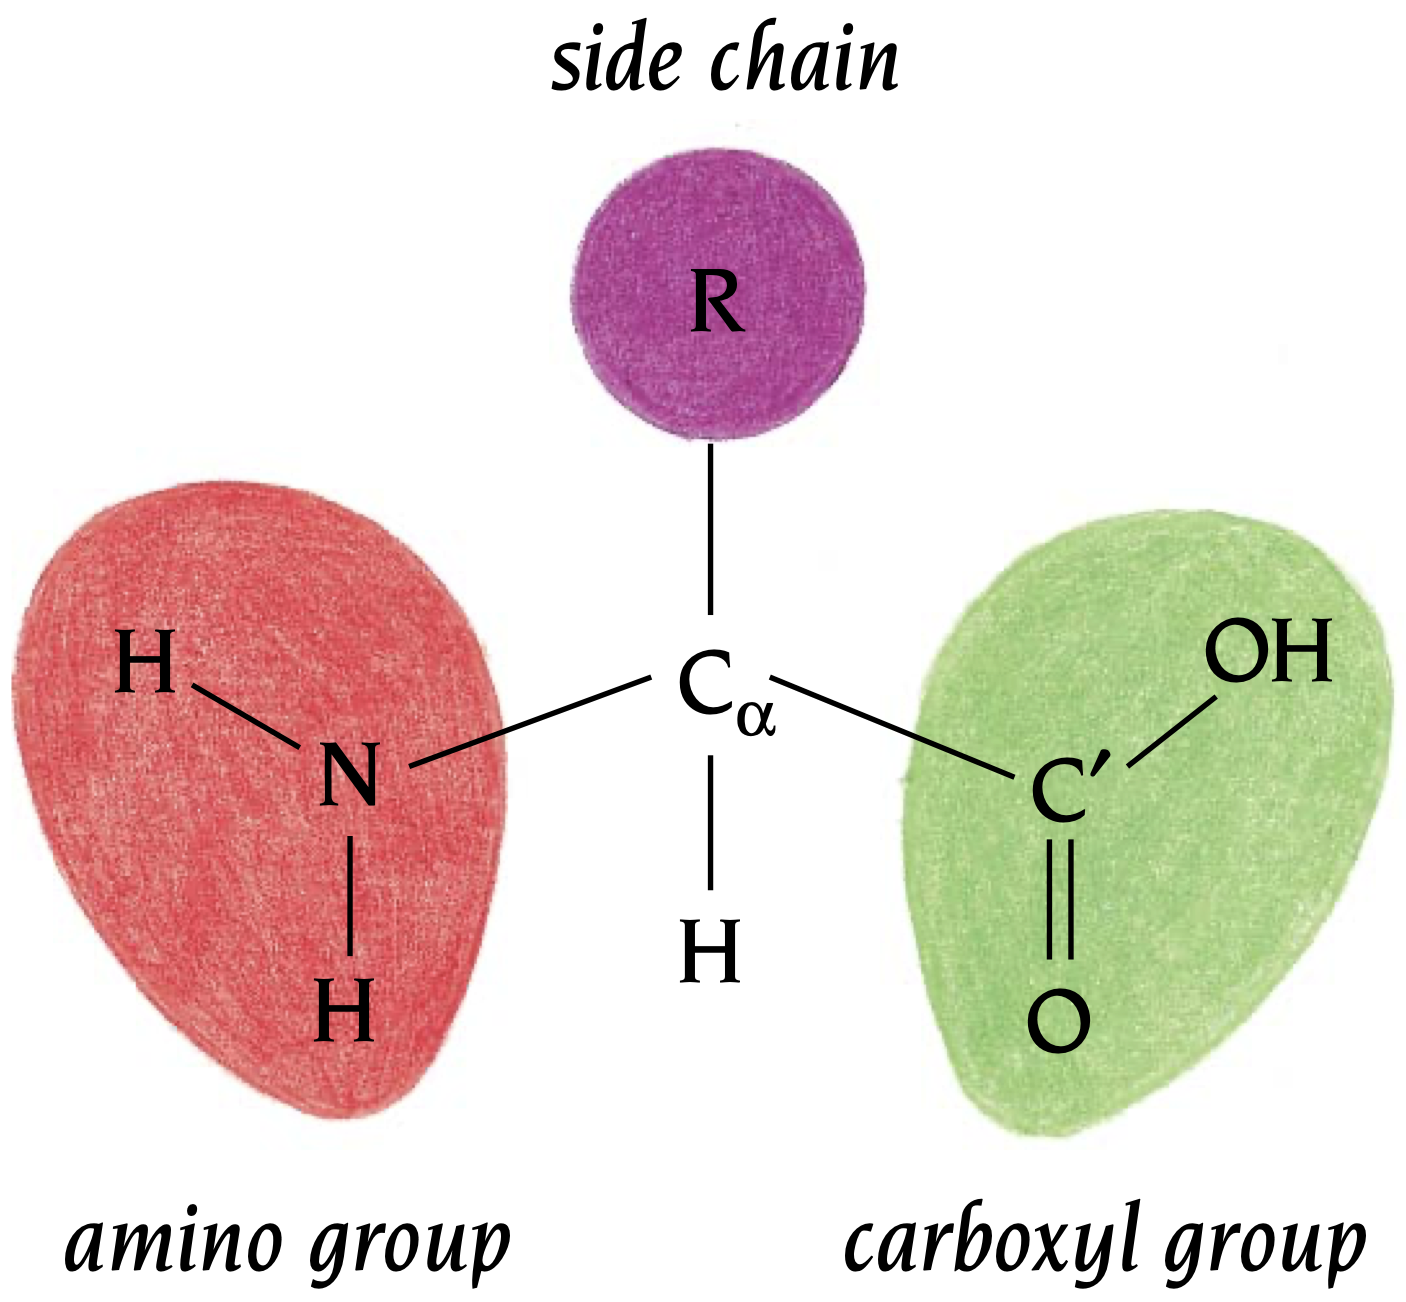
\includegraphics[width=\linewidth]{amino_acid.png}
        \caption{Amino acid}
        \label{fig:amino_acid}
    \end{subfigure}
    \begin{subfigure}[b]{0.75\textwidth}
        \centering
        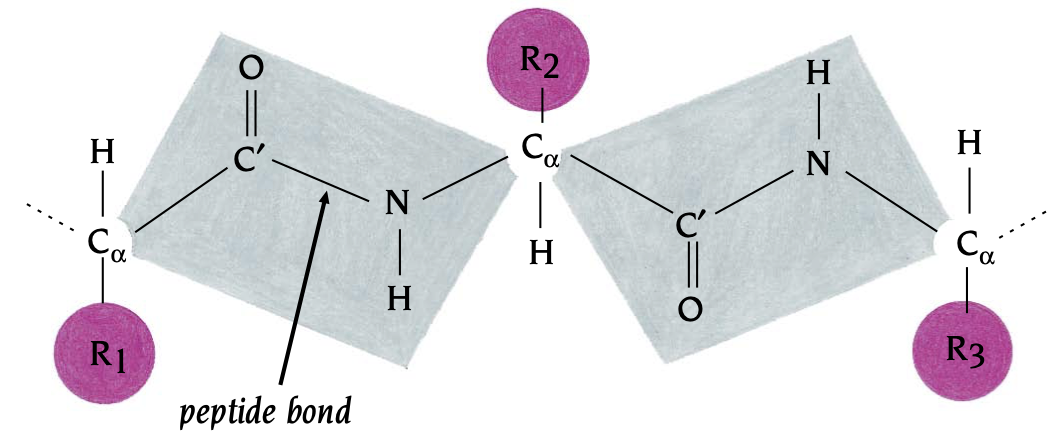
\includegraphics[width=\textwidth]{polypeptide_chain.png}
        \caption{Polypeptide chain}
        \label{fig:polypeptide_chain}
    \end{subfigure}
    \caption{Schematic diagram of an amino acid and polypeptide chain from \citet{branden2012IntroductionProteinStructure}. In this dissertation, we are interested only in the backbone formed by C\(_\alpha\) atoms.}
\end{figure}

Because the C\(_\alpha\) atoms define the backbone geometry of the chain, they provide a natural coarse-grained representation for structural modelling. In this work we adopt a C\(_\alpha\)-only representation: for a protein (chain of amino acid) \(x\) of length \(L\), each amino acid \(i \in \{1,\dots,L\}\) is associated with a 3D coordinate \(x^i \in \mathbb{R}^3\), so \(x\in\mathbb{R}^{L\times3}\). This coarse-grained representation is widely used in structural modelling because it captures global fold geometry and secondary structure while keeping the state space compact, making it well-suited to generative modelling \citep{watsonNovoDesignProtein2023,zhang2005TMalignProteinStructure,senior2020ImprovedProteinStructure}.

Even at this simplified level, protein geometry is far from arbitrary. The distance between successive C\(_\alpha\) atoms is consistently about
\begin{align*}
    \|x^i - x^{i-1}\| \approx 3.8~\text{\AA}.
\end{align*}
Local backbone conformation can be described by the angle formed by three consecutive C\(_\alpha\) atoms, \(\angle(x^{i-1}, x^i, x^{i+1})\), and by the dihedral angle defined by four consecutive C\(_\alpha\) atoms, \(\mathrm{dihedral}(x^{i-2}, x^{i-1}, x^i, x^{i+1})\). The empirically observed distributions of these geometric quantities are restricted by steric hindrance and the planarity of the peptide bond. Beyond these local constraints, valid structures must also avoid steric clashes, where non-adjacent amino acids are placed unrealistically close in space, and they typically fold into compact, physically plausible conformations \citep{creighton1993proteins,branden2012IntroductionProteinStructure}.

These intricate three-dimensional dependencies make protein backbones fundamentally different from unstructured data such as images or text. 
Consequently, generative models for proteins must account for spatial and structural constraints explicitly, motivating the use of geometry-aware representations and neural architectures.

\paragraph{Scope of this work.}
Our goal is backbone-level generative modelling using score-based diffusion. 
We do not impose hard geometric constraints during training or sampling (e.g.\ fixed bond lengths or bond angles); instead, we learn the distribution over C\(_\alpha\) coordinate trajectories and evaluate fidelity against native backbones. 
Section~\ref{sec:Experiments} reports RMSD/TM results and discusses the limitation that high RMSD or low TM can still correspond to physically valid but non-native folds.

\subsection{Graph Representation of Backbones}\label{subsec:graph-repr}
A protein backbone  of length \(L\) is represented as a graph \(G=(V,E)\), where each amino acid (or its corresponding C\(_\alpha\) atoms) corresponds to a node and edges capture both geometric proximity and sequential connectivity. This formulation enables the use of graph neural networks as score models, allowing information to be propagated through local neighbourhoods while respecting the spatial structure of the backbone. 

\paragraph{Nodes and node features.}
Each node \(i \in V\) corresponds to a amino acid with coordinate \(x^i \in \mathbb{R}^3\) representing the position of its C\(_\alpha\) atom. For simplicity, we do not include amino acid type or side-chain information in this work, focusing purely on the geometry of the C\(_\alpha\) atoms backbone. In addition to the coordinates (perturbation noises), extra node features are initialised as positional embeddings derived from the amino acid index (see \cref{subsec:architectures}, \cref{eq:positional-embedding}), along with time-conditioning features from the diffusion process (see \cref{subsec:architectures}, \cref{eq:time-embedding}). The full node feature vector is then obtained by concatenation:
\begin{align*}
    \text{Node feature} = \big[ \; \text{noises} \;\|\; \text{positional embedding} \;\|\; \text{time embedding} \;\big].
\end{align*}

\paragraph{Edges.}
Edges are constructed using a radius graph: for each node \(i\in V\), we connect edges to all neighbours \(j\) within a cutoff distance \(r\), subject to a maximum of \(k\) nearest neighbours. Formally,
\begin{align*}
    (i,j) \in E \quad \Leftrightarrow \quad \|x^i - x^j\| \leq r \quad \text{and}\quad j \text{ is among the } k \text{ closest to } i.
\end{align*}
This design ensures that local spatial relationships are captured without requiring a fixed sequence length. In addition to geometric edges, self-loops are included to stabilise message passing and allow each node to retain its own features. Edges are directed: for each \((i,j) \in E\), messages are passed from \(j\) (target) to \(i\) (source). This convention is consistent with the implementation in PyTorch Geometric, and we do not duplicate edges to create an undirected graph.

\paragraph{Edge features.}
For each edge \((i,j) \in E\), we compute a feature vector combining geometric and diffusion-time information. The feature vector includes the following:
\begin{itemize}
    \item \textbf{Radial basis encoding:} The distance \(\|x^i - x^j\|\) is expanded into a vector of length \(M\) using Gaussian radial basis functions,
        \begin{align*}
            \phi_\ell(\|x^i - x^j\|) = \exp\!\left(-\frac{(\|x^i - x^j\|-c_\ell)^2}{2\epsilon^2}\right),\quad \ell=1,...,M,
        \end{align*}
        where centres \(\{c_\ell\}_{\ell=1}^M\) are distributed uniformly between \(0\) and cutoff distance \(r\), length scale \(\epsilon=r/M\). This provides a smooth representation of distances. It is implemented via \texttt{e3nn.soft\_one\_hot\_linspace} from \citet{geiger2022E3nnEuclideanNeural,geiger2025EuclideanNeuralNetworks}.
    \item \textbf{Directional encoding:} The normalised vector
        \begin{align*}
            d^{\left(i,j\right)} = \frac{x^i - x^j}{\|x^i - x^j\|}\in \mathbb{R}^{3}
        \end{align*}
        encodes the relative orientation of the neighbour. This directional feature allows the network to capture local geometry beyond mere distances \citep{watsonNovoDesignProtein2023}.
    \item \textbf{Time embedding:} The diffusion timestep \(t\) is embedded into high-dimensional features (see \cref{subsec:architectures}, \cref{eq:time-embedding}) and projected through a linear layer. For each edge \((i,j)\), we associate the time embedding with the source node \(i\), enabling time-dependent conditioning of messages.
\end{itemize}
The full edge feature vector is then obtained by concatenation:
\begin{align*}
    h_{ij} = \big[ \;\phi_{1:M} \;\|\; d^{\left(i,j\right)},\,\forall \left(i,j\right)\in E \;\|\; \text{time embedding} \;\big].
\end{align*}

\paragraph{Rationale.}
This graph construction has several desirable properties: (i) it scales linearly with the number of amino acids (C\(_\alpha\) atoms) \(L\), (ii) it incorporates both distance and orientation information, which are critical for protein geometry, and (iii) it enables variable-length backbones to be handled naturally without padding. These features make it well-suited for score-based diffusion over protein structures.

\subsection{Score Models Architectures}\label{subsec:architectures}
The score network \(s_\theta(x,t)\) is parameterised by a neural network that maps noisy protein backbones to score estimates. We explore several architectures of increasing complexity, from a padding-based UNet model to a Graph Neural Network that utilises the graph representation.

\subsubsection{UNet Architecture on Padded Data}
As a baseline, we implemented a UNet architecture \citep{ronneberger2015UNetConvolutionalNetworks} with one dimensional convolutional neural networks applied directly to backbone coordinates represented as sequences of fixed length. Each protein was zero-padded to a common maximum length, and the UNet operated on the resulting coordinate tensors. This design provides a simple convolutional benchmark but does not handle variable-length inputs naturally and discards explicit geometric relationships between amino acids. It serves primarily as a sanity check to compare graph-based approaches against a conventional deep learning model.

\subsubsection{Graph Neural Network on Graph-Structured Data}\label{subsubsec:Transformer-GCN}
\paragraph{Graph Neural Networks.}
Neural networks can be extended to graph-structured data through Graph Neural Networks (GNNs) \citep{scarselliGraphNeuralNetwork2009,gilmer2017NeuralMessagePassing,battaglia2018RelationalInductiveBiases}. In this framework, each node updates its hidden representation by aggregating information, or messages, from its neighbours, typically following the generic message-passing scheme \citep{gilmer2017NeuralMessagePassing}:
\begin{align}\label{eq:GNN-message-passing}
    h_i^{(\ell+1)} \;=\; U\!\left(h_i^{(\ell)}, \; M\!\left(\left\{h_j^{(\ell)}, e_{ij} : j \in \mathcal{N}(i)\right\}\right)\right),
\end{align}
where \(h_i^{(\ell)}\) is the hidden state of node \(i\) at layer \(\ell\), \(\mathcal{N}(i)\) denotes its neighbourhood, \(e_{ij}\) are edge features, \(M\) is a function computing messages, and \(U\) is an update function that integrates messages into the node state.

One of the earliest and most widely used specialisations of this framework is the Graph Convolutional Network (GCN) \citep{kipf2017SemiSupervisedClassificationGraph}, which aggregates neighbour states through a normalised sum, analogous to convolution neural network (CNN). While effective, GCNs are limited in expressiveness, as they treat all neighbours uniformly and rely only on node features.

Subsequent work has introduced more expressive GNN variants. In this study we build on the Transformer-based graph convolution layer from \citet{shi2021MaskedLabelPrediction}, which enhances message passing by using an attention mechanism over both node and edge features. This allows the update in \cref{eq:GNN-message-passing} to assign different weights to different neighbours depending on their features, improving the ability of the model to capture the geometric and sequential structure of protein backbones. Specifically, the functions \(M\) and \(U\) in \cref{eq:GNN-message-passing} are defined via
\begin{align*}
    q_i \;&= W_q h_i^{(\ell)},\quad k_j = W_k h_j^{(\ell)}, \\
    \alpha_{ij}^{(\ell)} \;&=\; \mathrm{softmax}_{j \in \mathcal{N}(i)} 
    \big( q_i^{\top} (k_j + W_e e_{ij}) \big), \\
    h_i^{(\ell+1)} \;&=\; \sum_{j \in \mathcal{N}(i)} 
    \alpha_{ij}^{(\ell)} \, W_v h_j^{(\ell)},
\end{align*}
where \(e_{ij}\) is the edge feature vector, \(\alpha_{ij}^{(\ell)}\) are the attention weights, and \(W_q, W_k, W_e, W_v\) are learnable projections. In practice, multiple attention heads are computed in parallel and concatenated, but we present the single-head formulation for clarity. This formulation allows geometric encodings such as distances, orientations, and diffusion time embeddings to directly influence the attention weights, making the layer particularly well suited to protein backbone graphs.

\paragraph{Time conditioning via Gaussian Fourier features.}
Following \citet{song2021ScoreBasedGenerativeModeling}, we embed the diffusion time step \(t \in (0,1)\) using Gaussian Fourier features \citep{tancikFourierFeaturesLet2020}. Let \(d_{t}\) denote the dimension of time embedding, and let \(W \in \mathbb{R}^{d_{t}/2}\) have independent components \(W_k \sim \mathcal{N}(0,s^2)\) for \(k=1,...,d_{t}/2\). Then the embedding is defined by
\begin{align}\label{eq:time-embedding}
    \gamma(t) \;=\; \big[\, \cos(2\pi W t),\; \sin(2\pi W t)\,\big] \;\in \mathbb{R}^d_t,
\end{align}
where cosine and sine are applied elementwise. This provides a smooth and expressive encoding of time, allowing the score network to capture the evolution of noise levels across the diffusion process. In practice, \(\gamma(t)\) is passed through a shallow multi-layer perceptron (MLP) before being concatenated with node and edge features to condition the network on the current diffusion step.

\paragraph{Sinusoidal positional embeddings of amino acid indices.}
Graph-based models are inherently invariant to node permutations, which can be a limitation when modeling protein backbones where the sequential order of amino acids carries biologically meaningful directionality along the chain. To inject this ordering information, each node \(i \in \{1,\dots,L\}\) is assigned a normalized scalar index \(i/L \in (0,1]\). This scalar is mapped to a high-dimensional representation using sinusoidal positional encodings \citep{vaswaniAttentionAllYou2017},
\begin{align}\label{eq:positional-embedding}
    \rho(i) \;=\; \big[\, \sin(\omega_1 i/L),\; \cos(\omega_1 i/L),\; \dots,\; \sin(\omega_{d_i/2} i/L),\; \cos(\omega_{d_i/2} i/L)\,\big]\in\mathbb{R}^{d_i},
\end{align}
where \(d_i\) is the dimension of positional embedding, and \(\{\omega_k\}\) are fixed, exponentially spaced frequencies. The resulting positional embedding is passed through a shallow multi-layer perceptron (MLP) and concatenated with the initial node features, enabling the network to distinguish amino acids by their sequential position along the backbone.

\paragraph{Residual structure.}
Training deep graph networks is challenging because repeated aggregation can lead to oversmoothing of node representations and vanishing gradients \citep{li2018DeeperInsightsGraph,li2019DeepGCNsCanGCNs}. Residual connections \citep{he2016DeepResidualLearning} have since become a standard component of graph neural networks \citep{kipf2017SemiSupervisedClassificationGraph,li2019DeepGCNsCanGCNs}. They allow each layer to refine representations relative to the previous ones rather than completely replacing them, facilitating gradient flow through many stacked layers.

In this work we adopt a residual structure for every GNN block, so that the output of each layer is added to its input before passing through nonlinearities and normalisation. To further stabilise training, we employ GraphNorm \citep{cai2021GraphNormPrincipledApproach}, a normalisation technique specifically designed for graph neural networks. GraphNorm normalises node embeddings using graph-level statistics, improving convergence speed and reducing training instability compared to BatchNorm or LayerNorm. 

This combination of residual connections and GraphNorm improves optimisation stability, mitigates oversmoothing, and enables effective training of multi-layer architectures. Empirically, such designs have been shown to enhance performance on long chains and large graphs, which is particularly important in our setting of protein backbones where sequence lengths vary widely and capturing long-range dependencies is essential.
\begin{remark}
    The UNet baseline provides a simple non-graph benchmark. In practice, the inclusion of positional encodings has a noticeable effect on model quality. To quantify this contribution, we include a second baseline that employs the aforementioned GNN architecture without positional encodings. This variant captures local geometric neighbourhood information but lacks explicit representations of sequential order, thereby limiting its ability to model the directional structure of protein backbones.
\end{remark}

\subsection{Summary}\label{subsec:method-summary}
In this section we described the methodology for adapting score-based diffusion models to the task of protein backbone generation. We began by outlining the structural constraints of proteins and motivated the use of a C\(_\alpha\)-only representation. We then formulated backbones as graphs, with nodes corresponding to amino acids and edges defined through a radius neighbourhood, augmented by radial basis encodings, directional features, and diffusion-time embeddings. This representation captures geometric information in a permutation-invariant manner while naturally supporting variable-length backbones.

We constructed a graph neural network for the score network: a residual Transformer-based graph convolutional network with positional embeddings. The latter integrates geometric, sequential, and temporal information, supported by residual connections and GraphNorm.

The next section presents experimental results, benchmarking these models on the CATH S40 dataset using both quantitative metrics (RMSD, TM-score) and qualitative structural visualisations.

\clearpage

\section{Experiments}\label{sec:Experiments}
This section presents the experimental evaluation of the score-based diffusion models described in \cref{sec:SBD,sec:protein-gnn}. We benchmark three architectures on the CATH S40 dataset and assess their performance using quantitative metrics and qualitative visualisations. 

\subsection{Dataset}\label{subsec:dataset}
We train our models on the CATH S40 dataset \citep{orengo1997CATHHierarchicClassification,waman2024CATH2024CATHAlphaFlow,sillitoe2021CATHIncreasedStructural,lewis2018Gene3DExtensivePrediction}, a widely used benchmark for structural modelling tasks. The dataset clusters protein domains at \(40\%\) sequence identity, ensuring reduced redundancy while maintaining broad structural diversity. 

For each protein domain, we extract the backbone coordinates by retaining only the C\(_\alpha\) atom of each amino acid, yielding a variable-length sequence of coordinates \(\{x^i \in \mathbb{R}^3\}_{i=1}^L\), where \(L\) denotes the chain length, as mentioned in \cref{subsec:protein-structure}. The statistics of backbone lengths is summarised in \cref{tab:cath-stats}. Backbones are then converted into graphs as described in \cref{subsec:graph-repr}, and coordinates are normalised prior to training.

\begin{table}[htbp]
    \centering
    \caption{Summary statistics of backbone lengths in the CATH S40 dataset.}
    \label{tab:cath-stats}
    \begin{tabular}{lccccc}
        \toprule
        & Min & Max & Mean & Median & Std \\
        \midrule
        Length (\(L\)) & 11 & 1202 & 155 & 133 & 89 \\
        \bottomrule
    \end{tabular}
\end{table}

\subsection{Training and Sampling}
\paragraph{Training setup.}
For the forward noising process we adopt the variance-preserving (VP) SDE formulation (\cref{eq:VPSDE}) with the cosine noise schedule (\cref{eq:cosine-beta}). The training objective is the denoising score matching loss (\cref{eq:DSM}), optimising the score networks described in \cref{subsec:architectures}. Models are trained using the Adam optimiser \citep{kingma2017AdamMethodStochastic} with a batch size dynamically adapted to GPU memory constraints.

\paragraph{Sampling.}
New backbone structures are generated by simulating the reverse SDE using predictor-corrector (PC) sampling, starting from Gaussian noise (\cref{sec:PC-sampling}). This procedure enables diverse yet structurally plausible backbone generations.

\paragraph{Implementation.}
All models are implemented in Python using PyTorch and PyTorch Geometric \citep{PyG1.0,PyG2.0}. 
Experiments were conducted on NVIDIA GPUs with 48GB memory.

\subsection{Evaluation Metrics}\label{subsec:metrics}
We evaluate reconstruction fidelity using two widely adopted measures of structural similarity: root-mean-square deviation (RMSD) and TM-score.

\paragraph{Root-mean-square deviation (RMSD).}
RMSD provides a direct measure of average atomic displacement between two aligned structures. 
Given a generated backbone \(X=\{x_i\}_{i=1}^L\) and its reference \(Y=\{y_i\}_{i=1}^L\), 
the RMSD is defined as
\begin{align*}
    \mathrm{RMSD}(X, Y) \;=\; \sqrt{\frac{1}{L}\sum_{i=1}^{L} \|x_i - y_i\|^2}.
\end{align*}
Lower values indicate closer correspondence to the reference. 
Although widely used, RMSD can be overly sensitive to local misalignments, 
and large deviations in one region may dominate the score even if the overall fold is preserved.

\paragraph{TM-align and TM-score.}
To complement RMSD, we use TM-score \citep{zhang2004ScoringFunctionAutomated,xu2010HowSignificantProtein}, a structural similarity measure in \((0,1]\), computed via the TM-align algorithm \citep{zhang2005TMalignProteinStructure}. Unlike RMSD, TM-score is less affected by local errors and more reflective of global fold similarity. In practice, TM-align performs a sequence-independent superposition of two protein structures using heuristic dynamic programming, returning both an optimal alignment and the corresponding TM-score. Interpretation of TM-scores follows established conventions: values below \(0.2\) typically correspond to unrelated structures, while scores above \(0.5\) generally indicate that two proteins share the same overall fold within SCOP/CATH classification. Thus, TM-score serves as a more robust global measure of structural fidelity and complements RMSD in our evaluation.

\begin{remark}
    Because each generated backbone is compared to its specific native target of the same length \(L\), RMSD and TM-score measure reconstruction fidelity, not absolute physical validity. This is appropriate for our benchmarking setting (paired evaluation), but one should interpret low TM or high RMSD with caution: a generated backbone may still represent a plausible alternative fold while scoring poorly against the chosen reference.
\end{remark}

\subsection{Quantitative Results}\label{subsec:results}
We benchmarked three model variants: (i) a UNet baseline on padded coordinate 
sequences, (ii) a Transformer-based graph convolutional network with and without positional 
encodings, as detailed in \cref{subsec:architectures}. Evaluation was performed using RMSD and TM-score, as described in \cref{subsec:metrics}.

\paragraph{Overall performance.}
The summary statistics of overall performance is reported in \cref{tab:quant-results}. From the results, the Transformer-based graph convolutional network with positional encodings achieves the best overall performance, with the lowest RMSD (\(16.39 \pm 4.29\) \AA) and highest TM-score (\(0.272 \pm 0.041\)). By contrast, the same architecture without positional encodings performs substantially worse, highlighting the importance of incorporating sequential information in addition to geometric neighbourhoods. Interestingly, the UNet baseline outperforms the GCN without positional encodings, despite its simplistic design and reliance on padded sequences. This suggests that while graph representations capture local geometry, they require positional encodings to effectively model the directional structure of protein backbones.

\begin{table}[htbp]
    \centering
    \caption{Quantitative evaluation of backbone reconstruction fidelity. 
    Values reported are mean \(\pm\) standard deviation.}
    \label{tab:quant-results}
    \begin{tabular}{lcc}
        \toprule
        Model & RMSD (\AA) & TM-score \\
        \midrule
        UNet baseline & \(17.230 \pm 4.699\) & \(0.264 \pm 0.041\) \\
        GCN w/o positional encoding & \(20.459 \pm 4.985\) & \(0.145 \pm 0.023\) \\
        GCN w/ positional encoding & \(16.394 \pm 4.294\) & \(0.272 \pm 0.041\) \\
        \bottomrule
    \end{tabular}
\end{table}

\paragraph{Distribution analysis.}
In addition to summary statistics, we plot the distribution plot and box plot of RMSD and TM-scores across the dataset, \cref{fig:rmsd-dist-box-plot,fig:tm-dist-box-plot}. These results reinforce the trends observed in \cref{tab:quant-results}. The GCN model with positional encodings exhibits the most favourable distribution, with RMSD values concentrated toward lower errors and TM-scores shifted toward higher similarity. The UNet baseline, although simpler, produces a broader distribution with a heavier tail of poorly reconstructed examples. By contrast, the GCN without positional encodings consistently underperforms, with TM-scores clustered around low values and RMSD heavily shifted left, demonstrating that sequential information is critical for modelling backbone geometry.

\begin{figure}[htbp]
    \centering
    \begin{subfigure}[b]{0.57\textwidth}
        \centering
        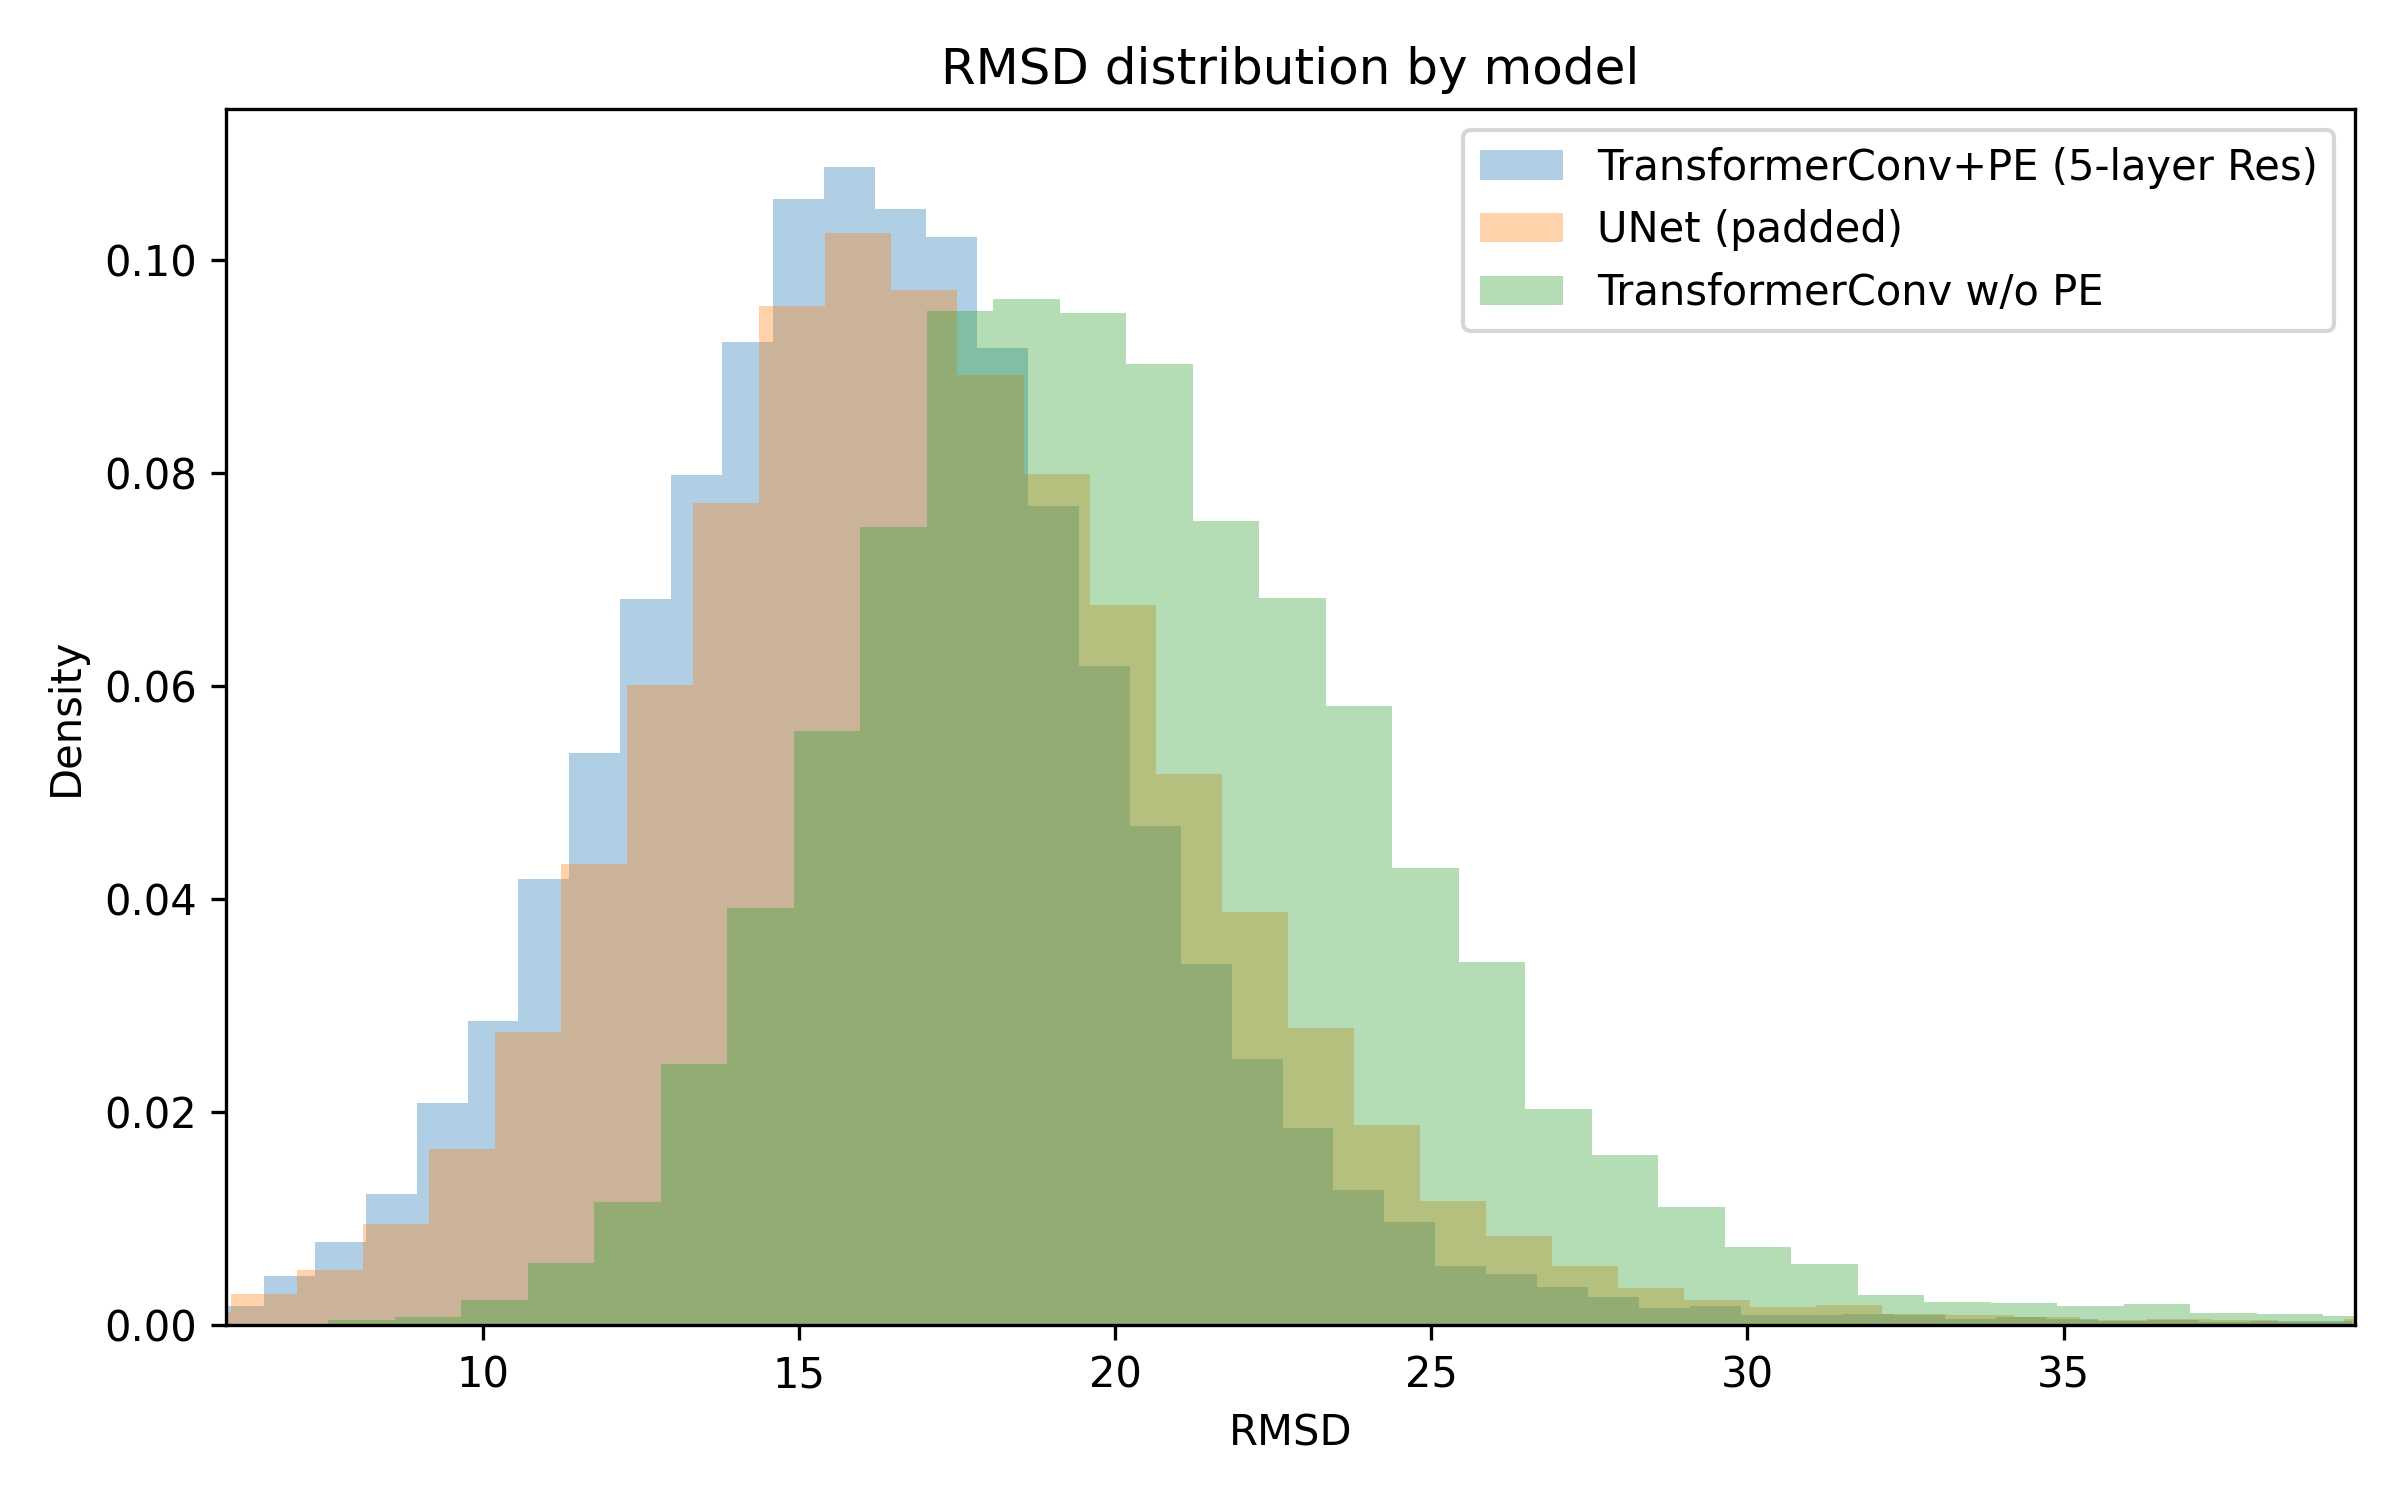
\includegraphics[width=\linewidth]{rmsd_dist.png}
        \caption{Distribution of RMSD.}
        \label{fig:rmsd-hist}
    \end{subfigure}
    \begin{subfigure}[b]{0.42\textwidth}
        \centering
        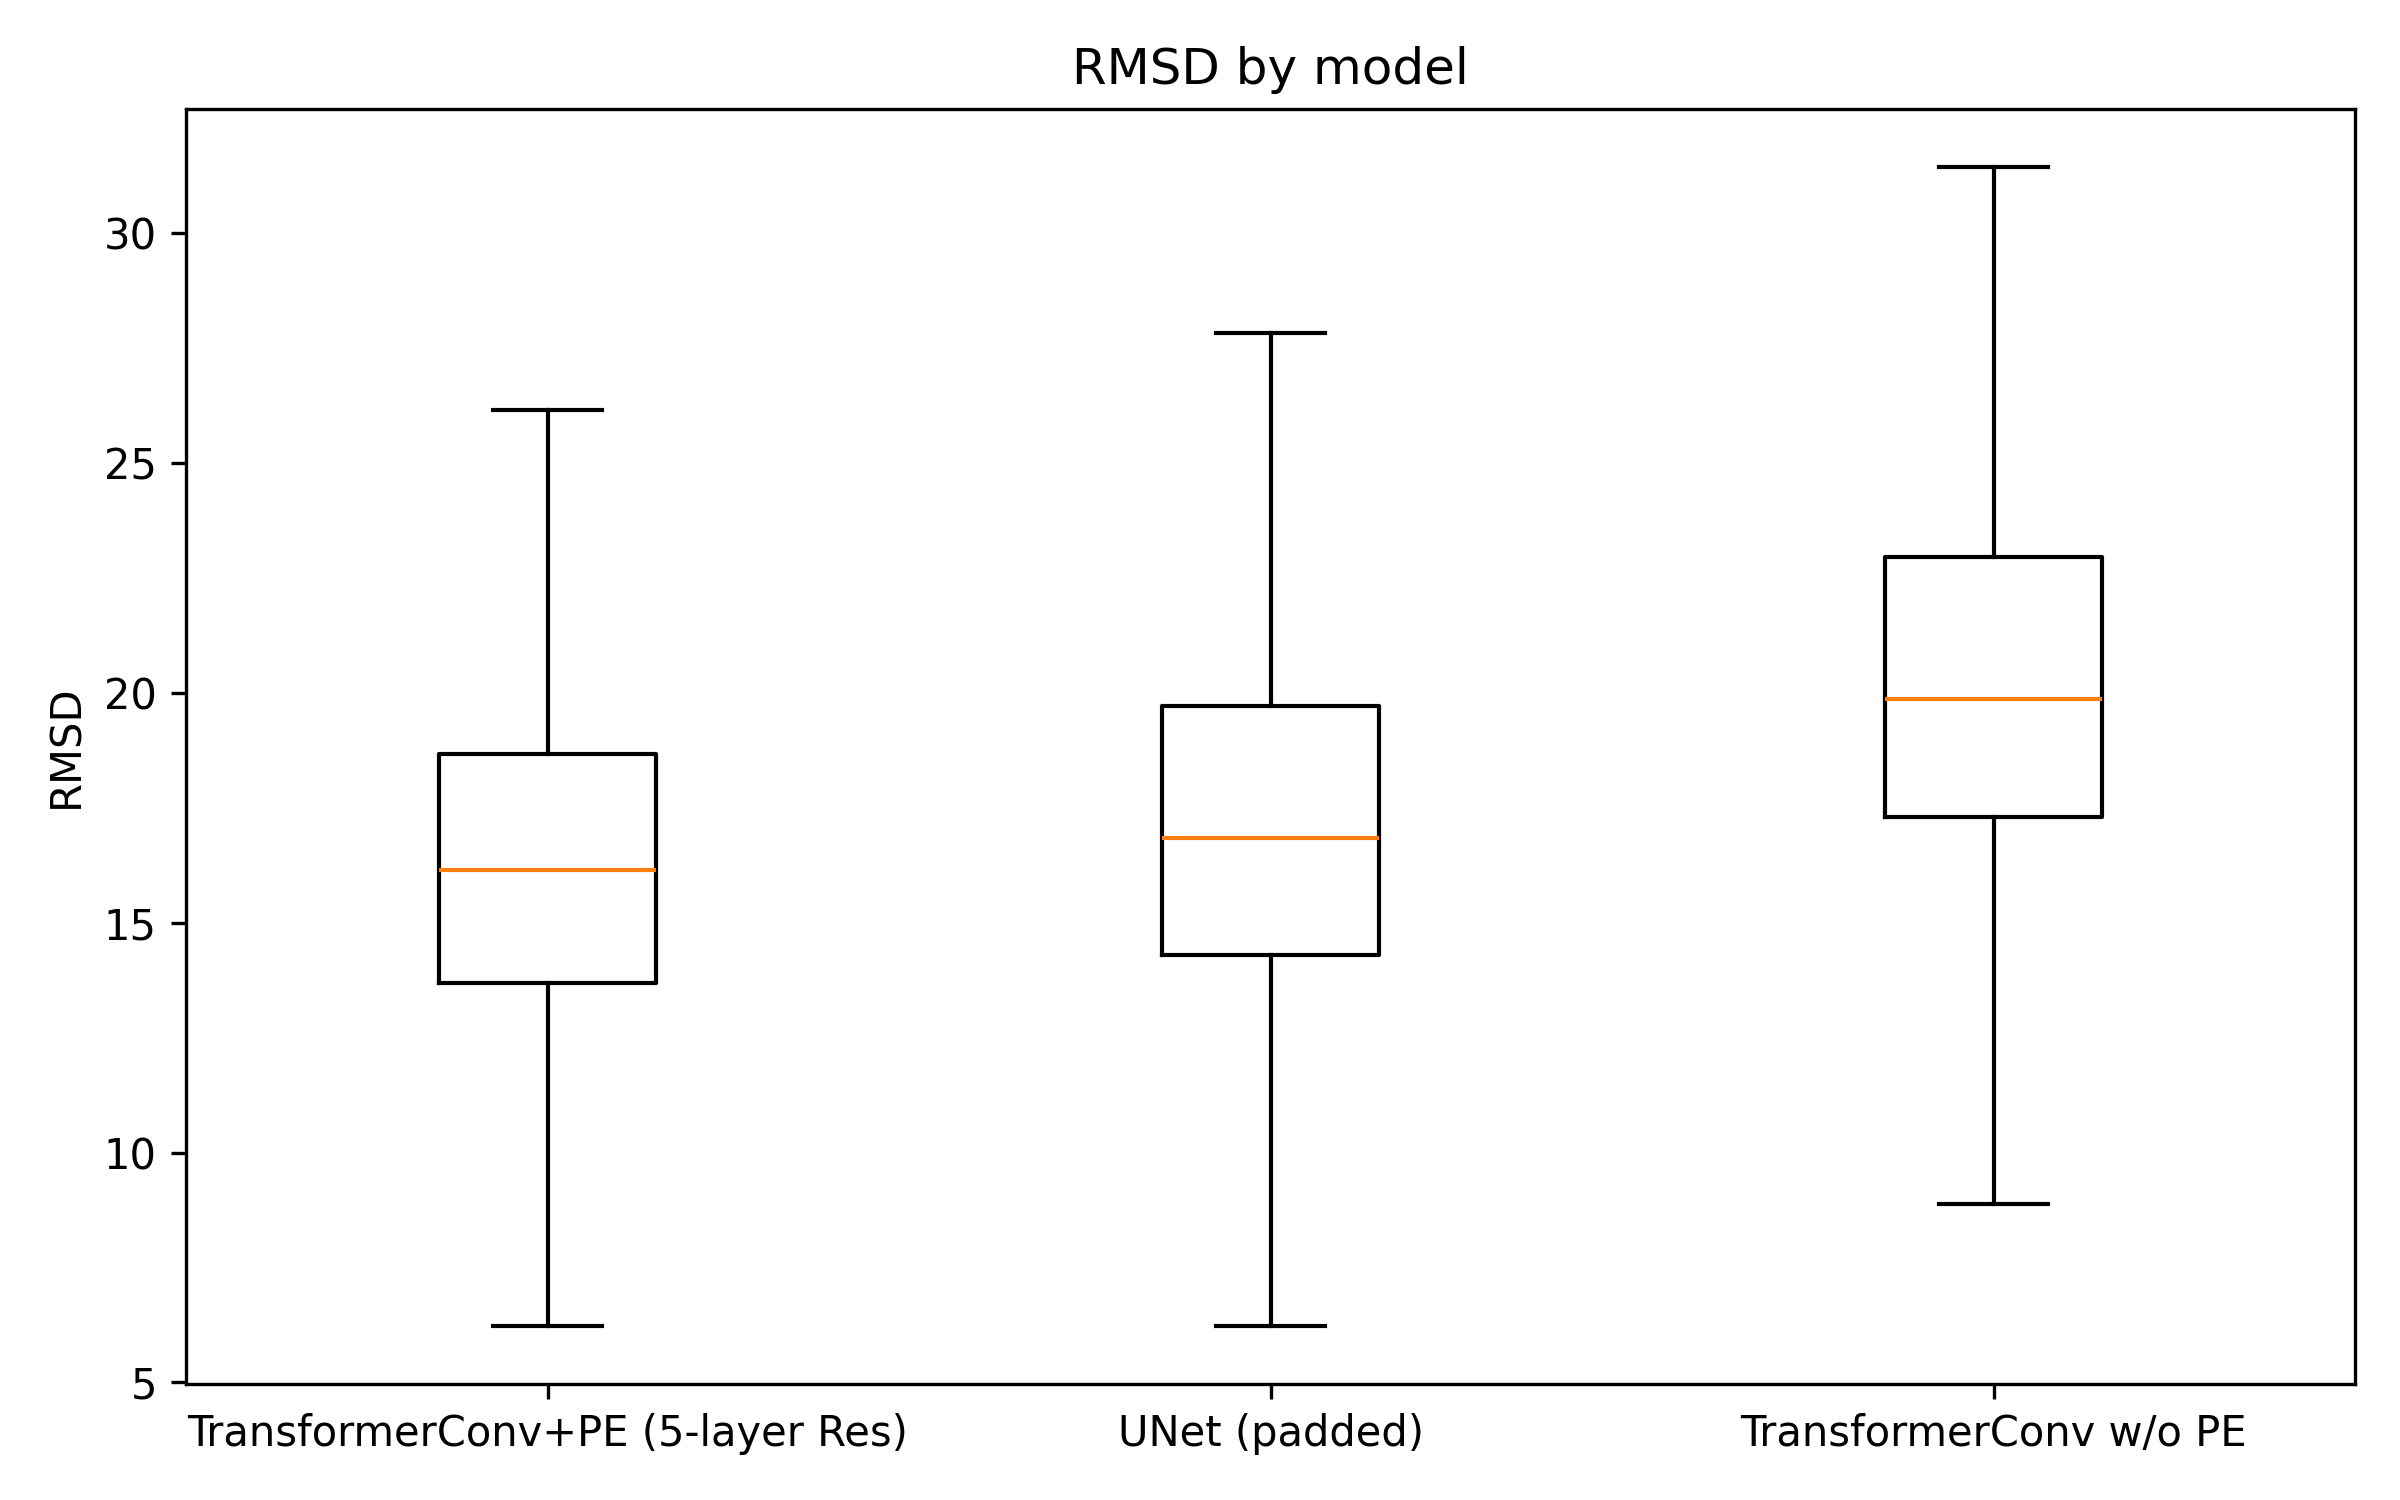
\includegraphics[width=\linewidth]{rmsd_box.png}
        \caption{Box plot of RMSD.}
        \label{fig:rmsd-box}
    \end{subfigure}
    \caption{Distribution and box plot of RMSD values across test structures. Lower is better.}
    \label{fig:rmsd-dist-box-plot}
\end{figure}

\begin{figure}[htbp]
    \centering
    \begin{subfigure}[b]{0.57\textwidth}
        \centering
        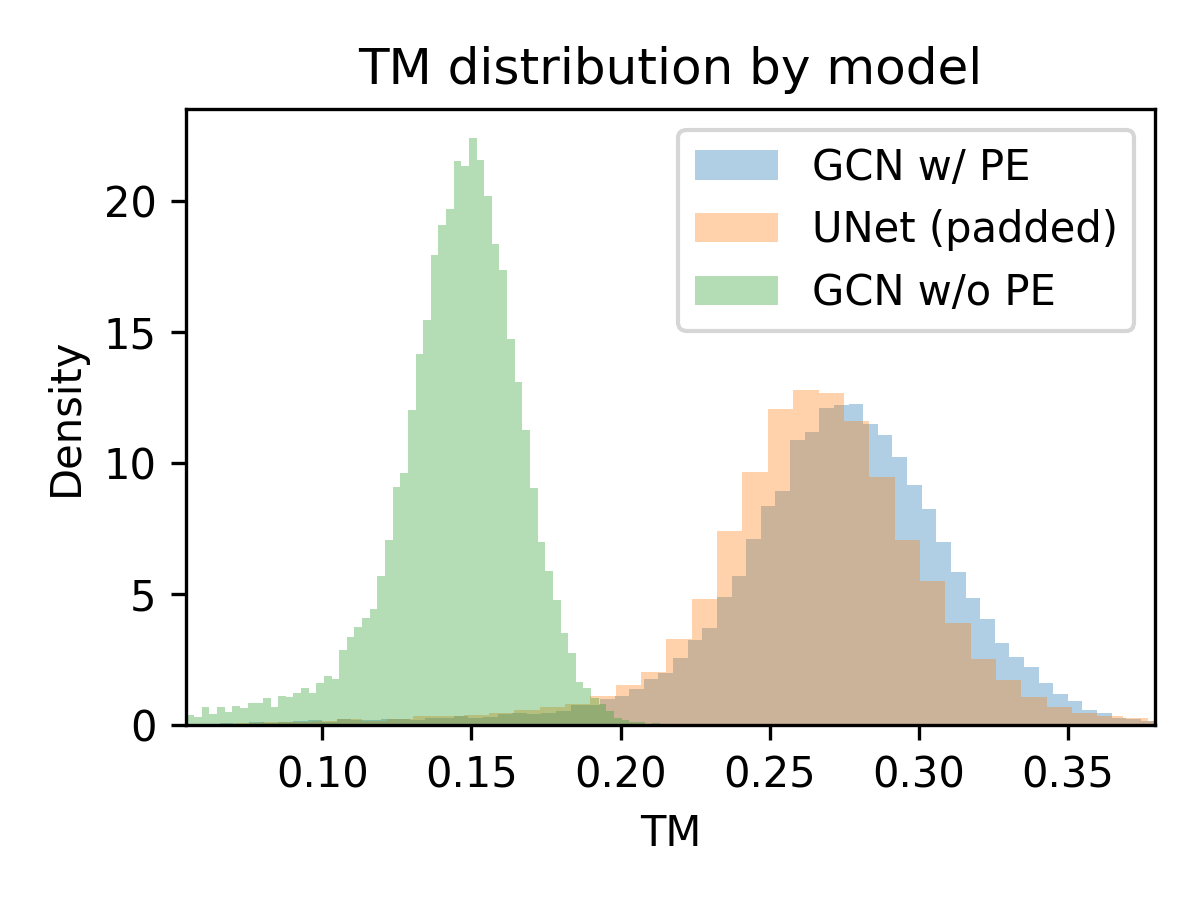
\includegraphics[width=\linewidth]{tm_dist.png}
        \caption{Distribution of TM-score.}
        \label{fig:tm-hist}
    \end{subfigure}
    \begin{subfigure}[b]{0.42\textwidth}
        \centering
        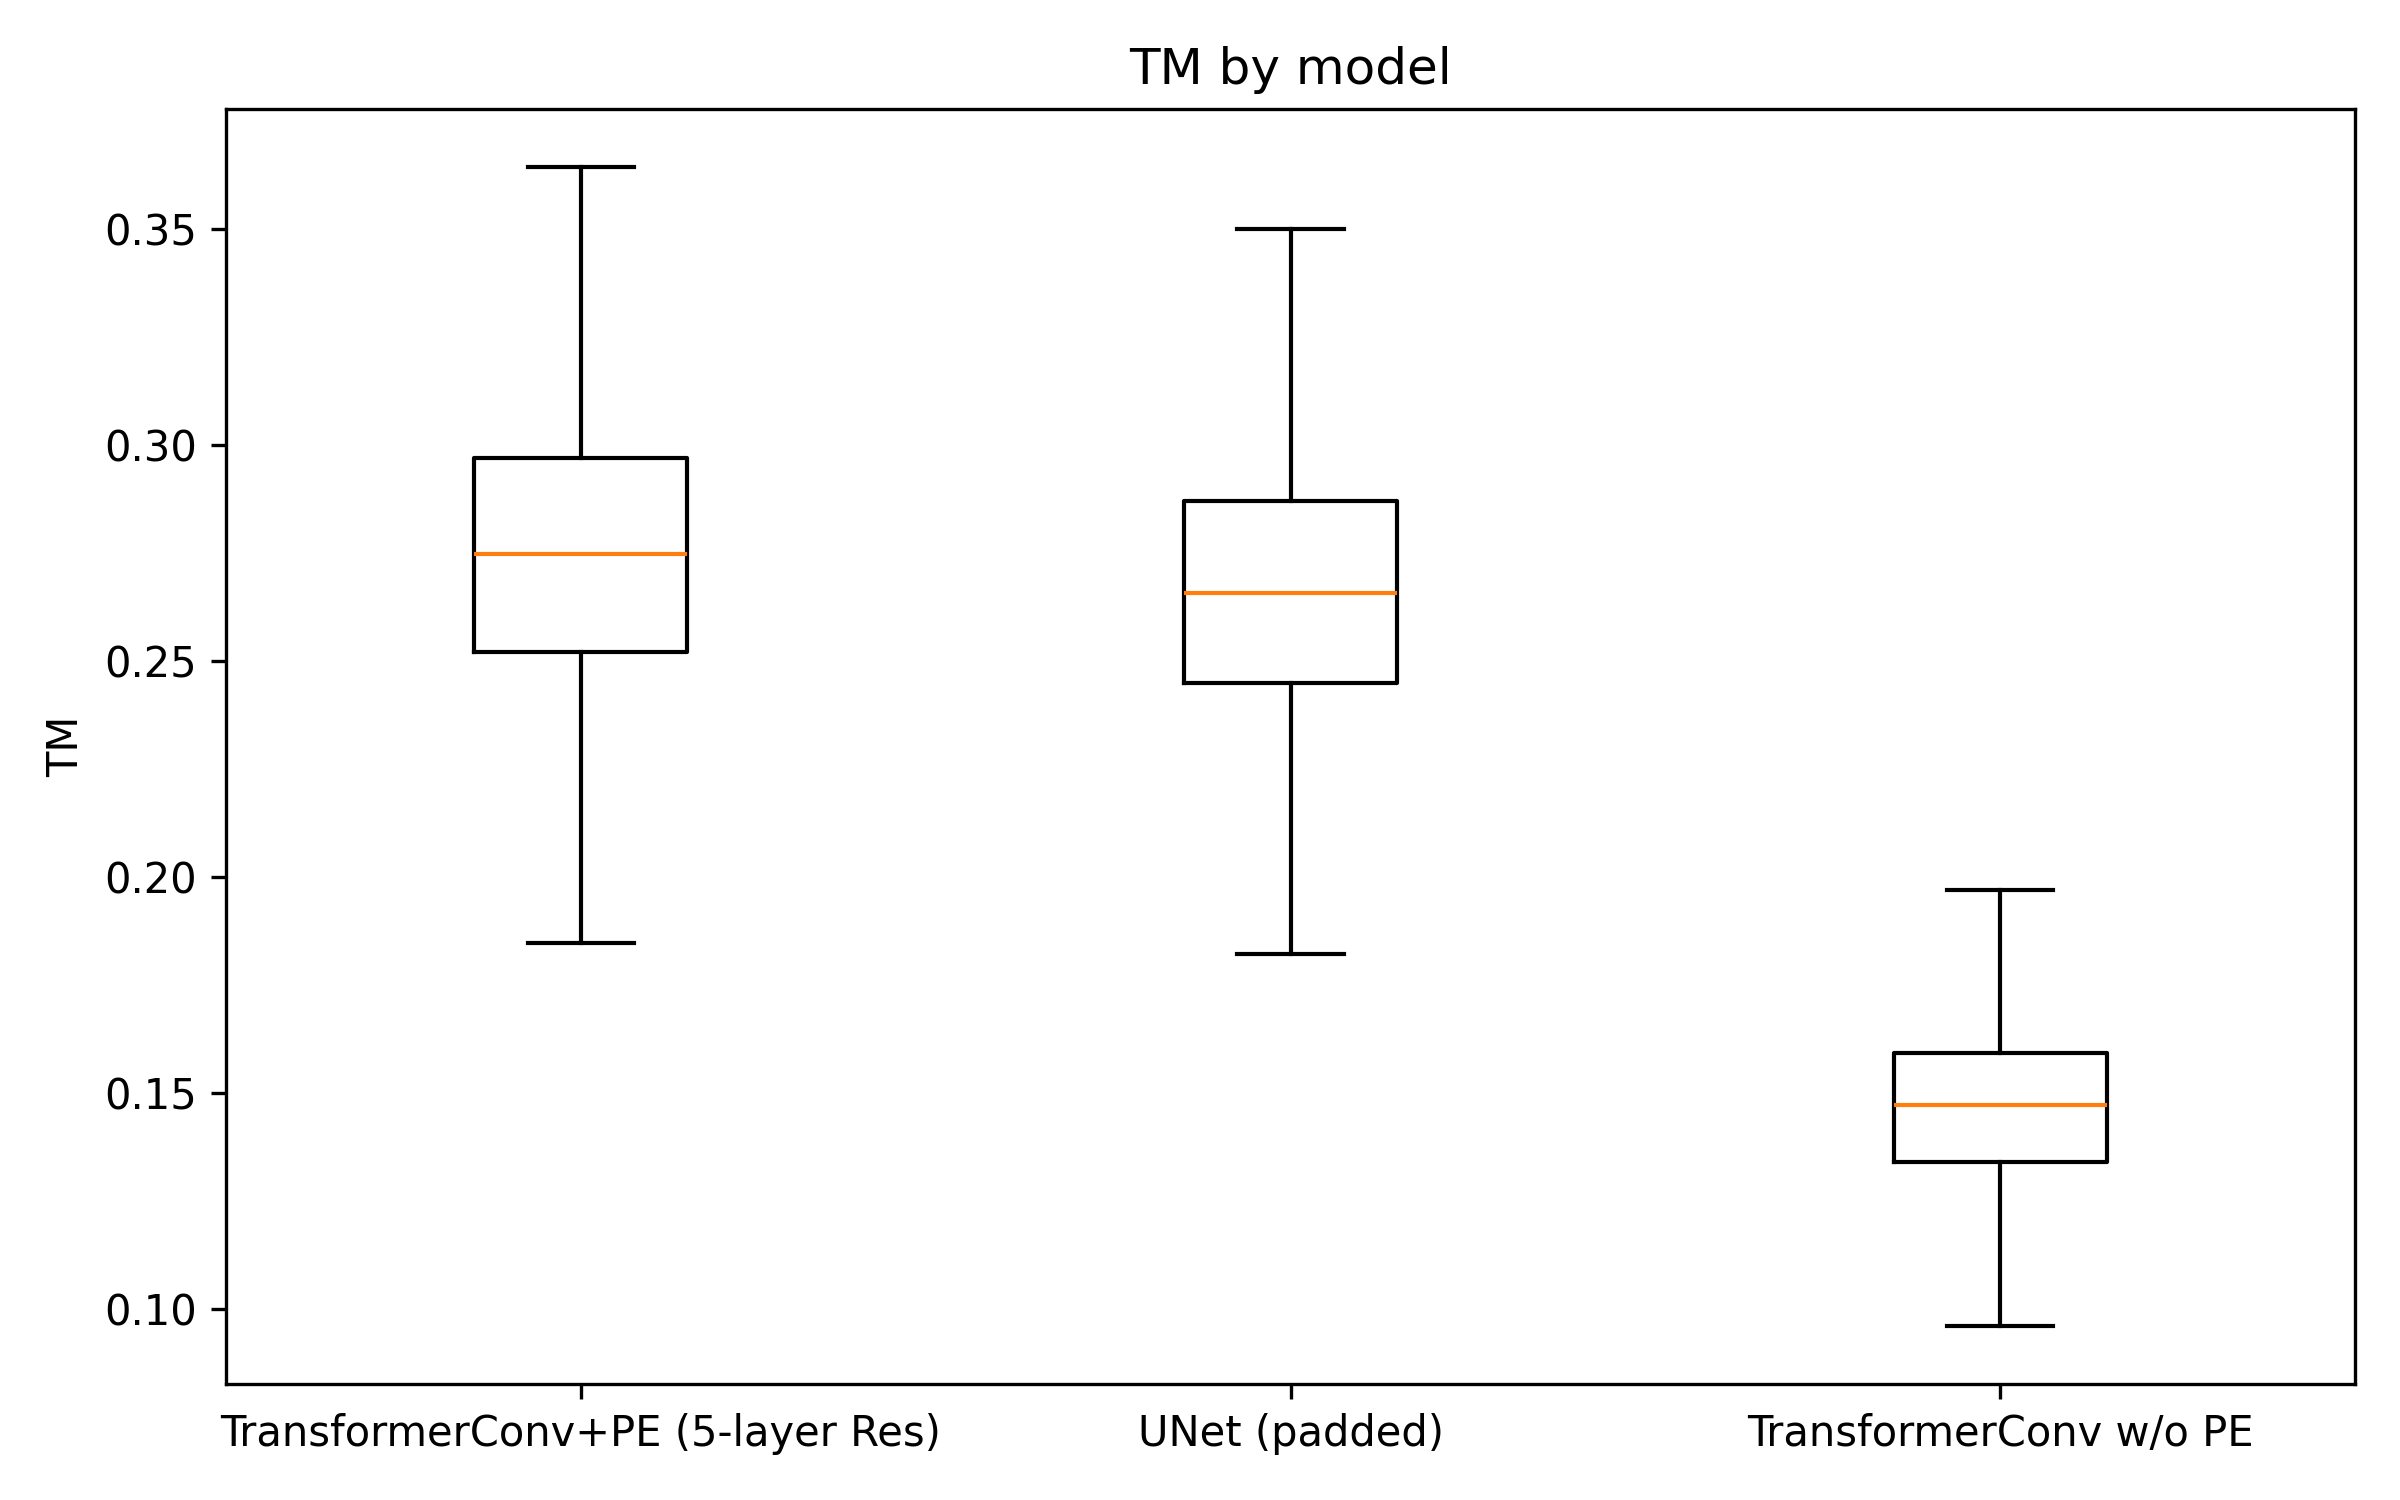
\includegraphics[width=\linewidth]{tm_box.png}
        \caption{Box plot of TM-score.}
        \label{fig:tm-box}
    \end{subfigure}
    \caption{Distribution and box plot of TM-scores across test structures. Higher is better.}
    \label{fig:tm-dist-box-plot}
\end{figure}

We further analyse model performance as a function of backbone length \(L\), plotting RMSD and TM-score versus \(L\) in \cref{fig:rmsd-tm-vs-l}. Both metrics exhibit a clear dependence on sequence length: reconstruction error (RMSD) increases with \(L\), while TM-score tends to decrease for longer proteins. This trend reflects the inherent difficulty of maintaining structural fidelity over extended chains, where deviations accumulate and long-range dependencies become harder to capture.

\begin{figure}[htbp]
    \centering
    \begin{subfigure}[b]{0.495\textwidth}
        \centering
        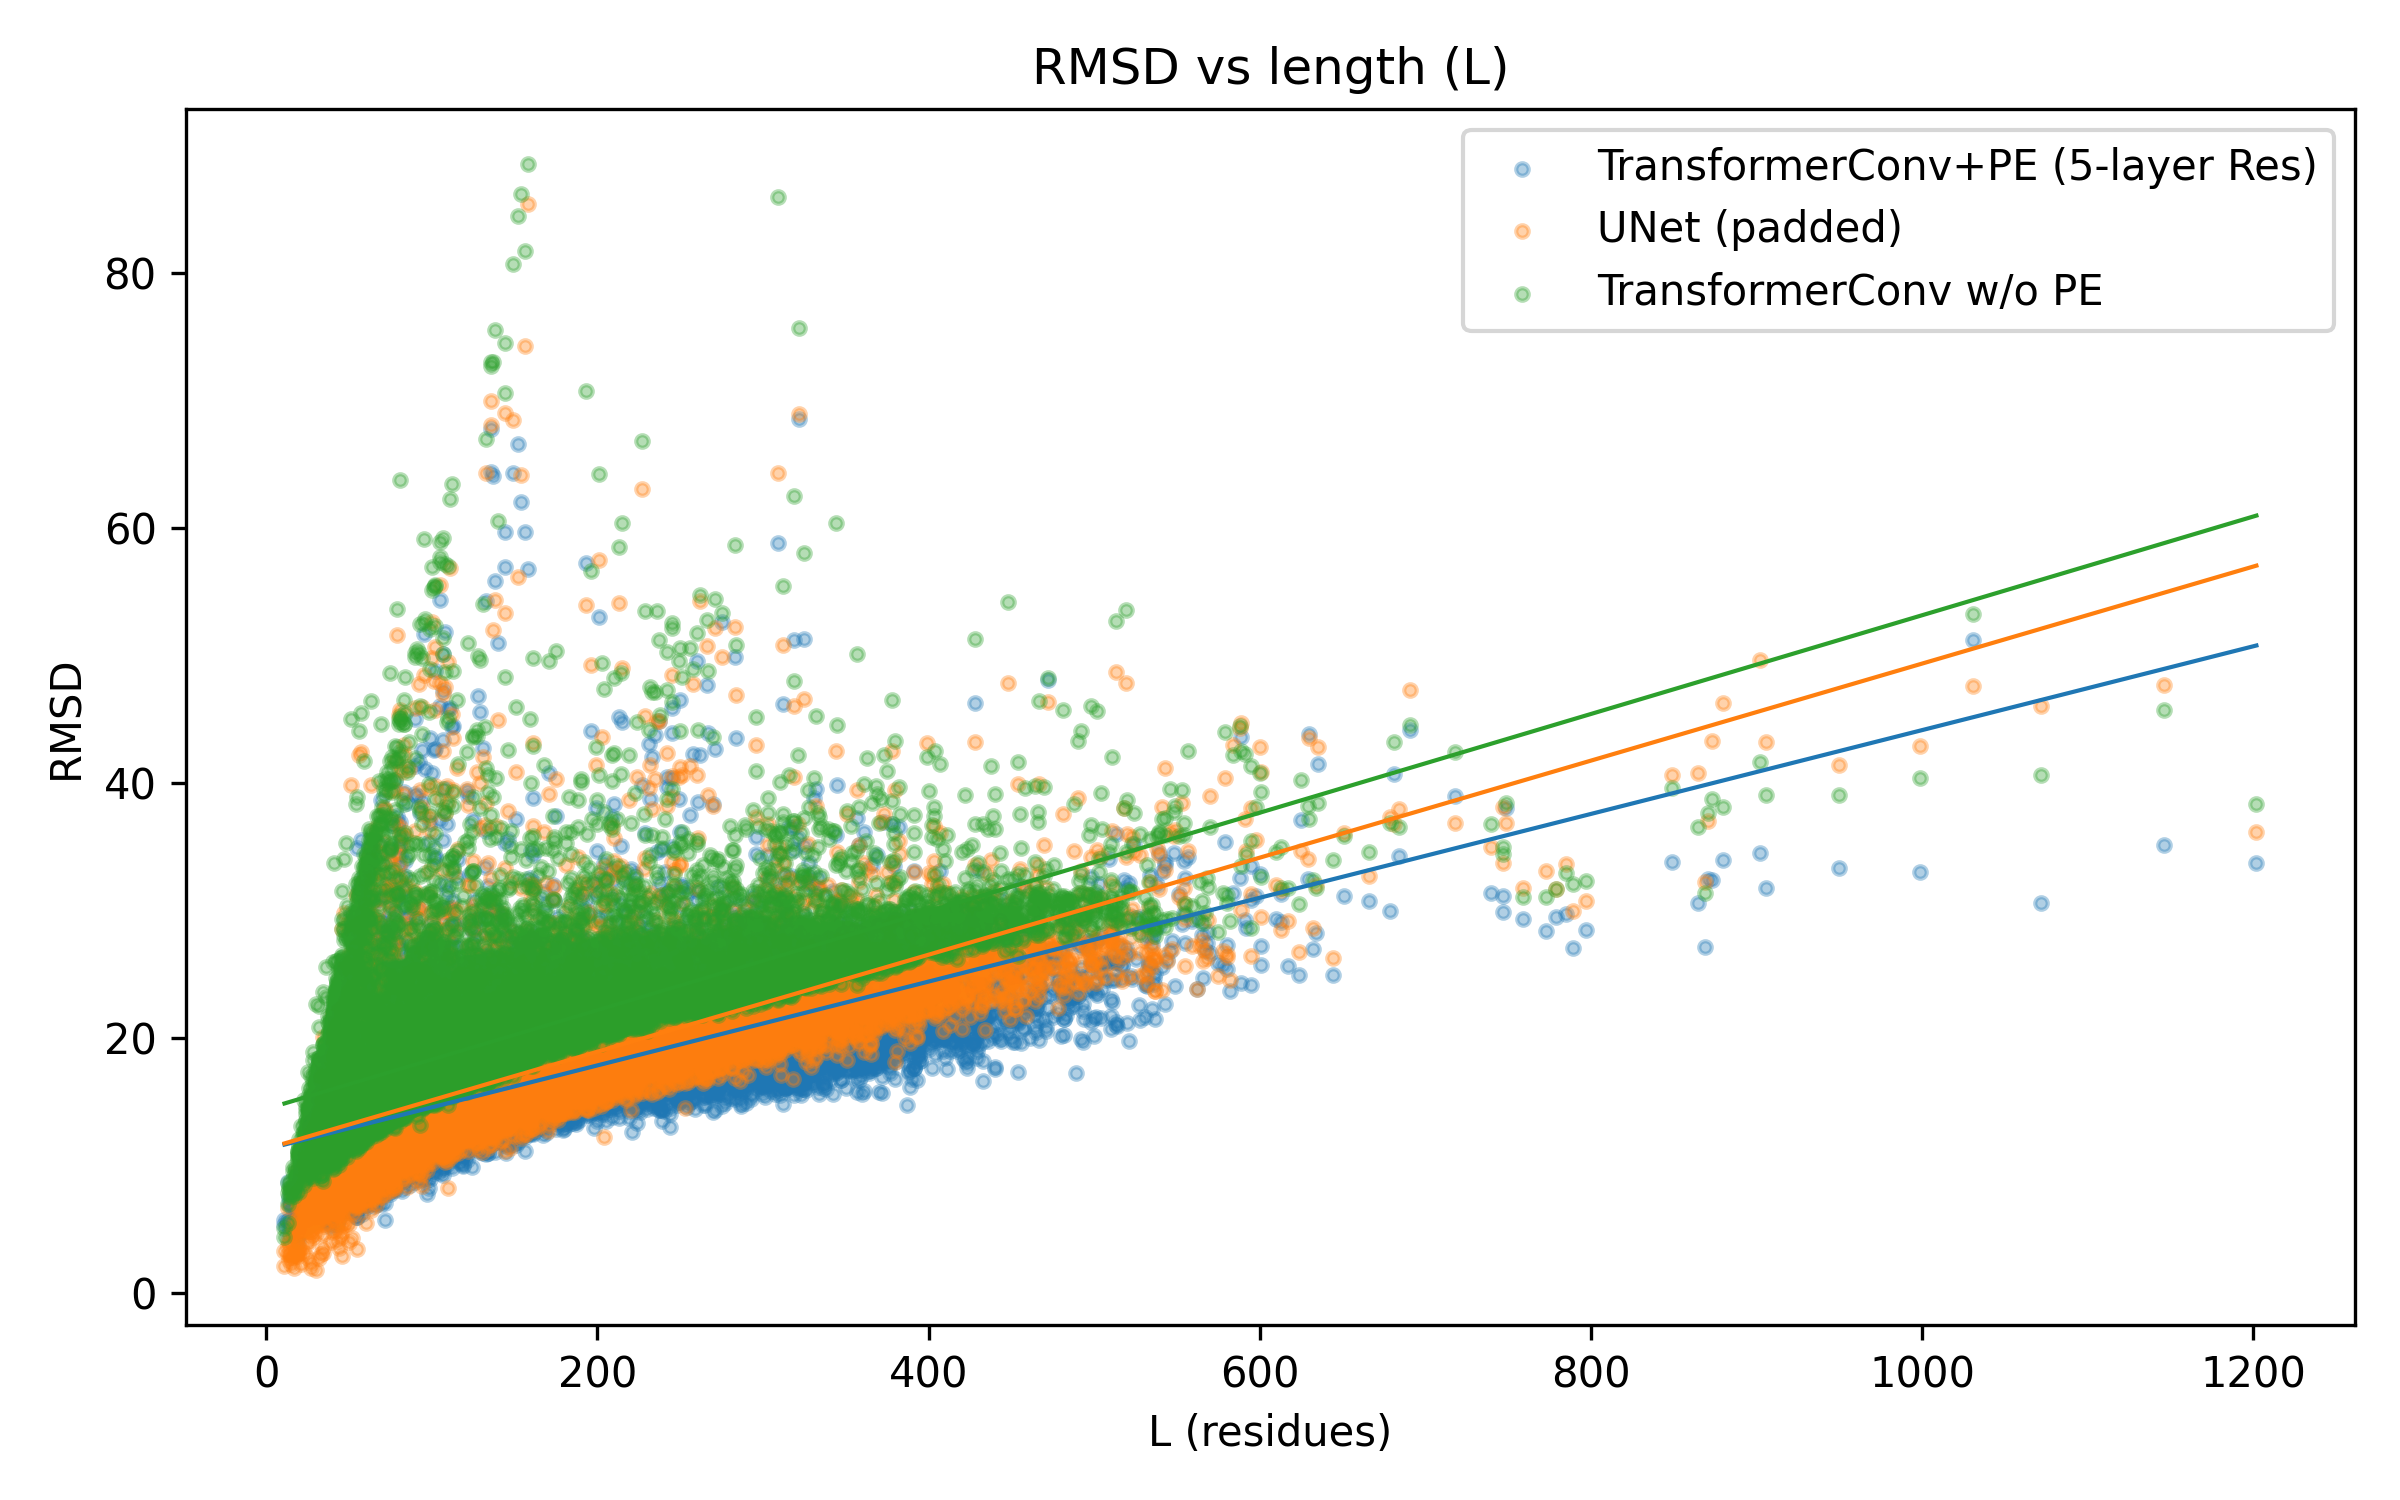
\includegraphics[width=\linewidth]{rmsd_vs_L.png}
        \caption{RMSD vs. \(L\).}
        \label{fig:rmsd-vs-l}
    \end{subfigure}
    \begin{subfigure}[b]{0.495\textwidth}
        \centering
        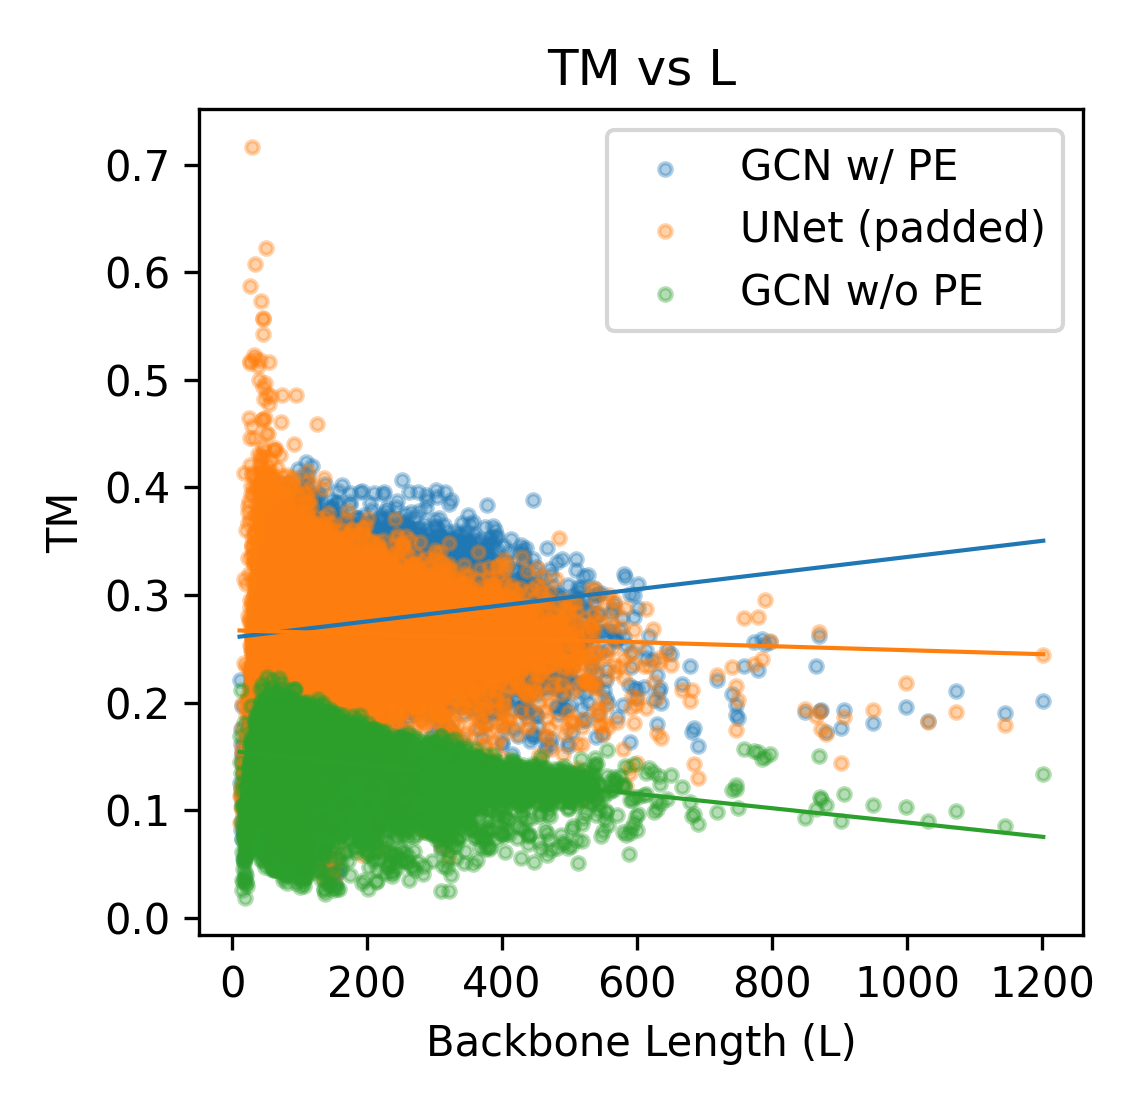
\includegraphics[width=\linewidth]{tm_vs_L.png}
        \caption{TM-score vs. \(L\).}
        \label{fig:tm-vs-l}
    \end{subfigure}
    \caption{RMSD and TM-score versus backbone length \(L\).}
    \label{fig:rmsd-tm-vs-l}
\end{figure}

Across all lengths, the GCN model with positional encodings achieves the best performance, with lower RMSD growth rates and consistently higher TM-scores. The UNet baseline performs comparably on shorter backbones but degrades more quickly as length increases, consistent with its reliance on fixed-length padded representations. The GCN without positional encodings consistently underperforms, with rapidly increasing RMSD and TM-scores falling below \(0.2\) for most lengths, highlighting its inability to capture directional structure. These results emphasise that positional encodings are particularly critical for modelling long backbones, where sequential information provides essential constraints on geometry.

\subsection{Qualitative Visualisation}\label{subsec:visualisation}
We now present qualitative visualisations of generated backbones alongside a true native backbone, rendered in PyMOL \citep{PyMOL,JyMOL,AxPyMOL}. For each case, we display the C\(_\alpha\)-trace of the generated structure together with the corresponding reference backbone (\cref{fig:samples}). These visualisations provide an intuitive sense of how different architectures behave, illustrate both successful reconstructions, where the generated backbone closely follows the native fold (low RMSD, high TM-score), and failure cases, where the model produces geometrically plausible but non-native conformations.

The Transformer-based GCN with positional encodings produces generations that resemble the overall topology of the reference backbone, though with local deviations. The UNet baseline yields broadly plausible structures but can introduce artifacts, particularly in regions affected by padding. The GCN without positional encodings performs noticeably worse in this example, 
producing a collapsed global fold. While these individual cases are not sufficient for firm conclusions, they are broadly consistent with the quantitative trends: positional information improves global fold recovery, and its absence leads to systematic degradation. Together, these visualisations complement the statistical results by illustrating the kinds of conformations the models tend to generate.

\begin{figure}[htbp]
    \centering
    \begin{subfigure}[b]{0.495\textwidth}
        \centering
        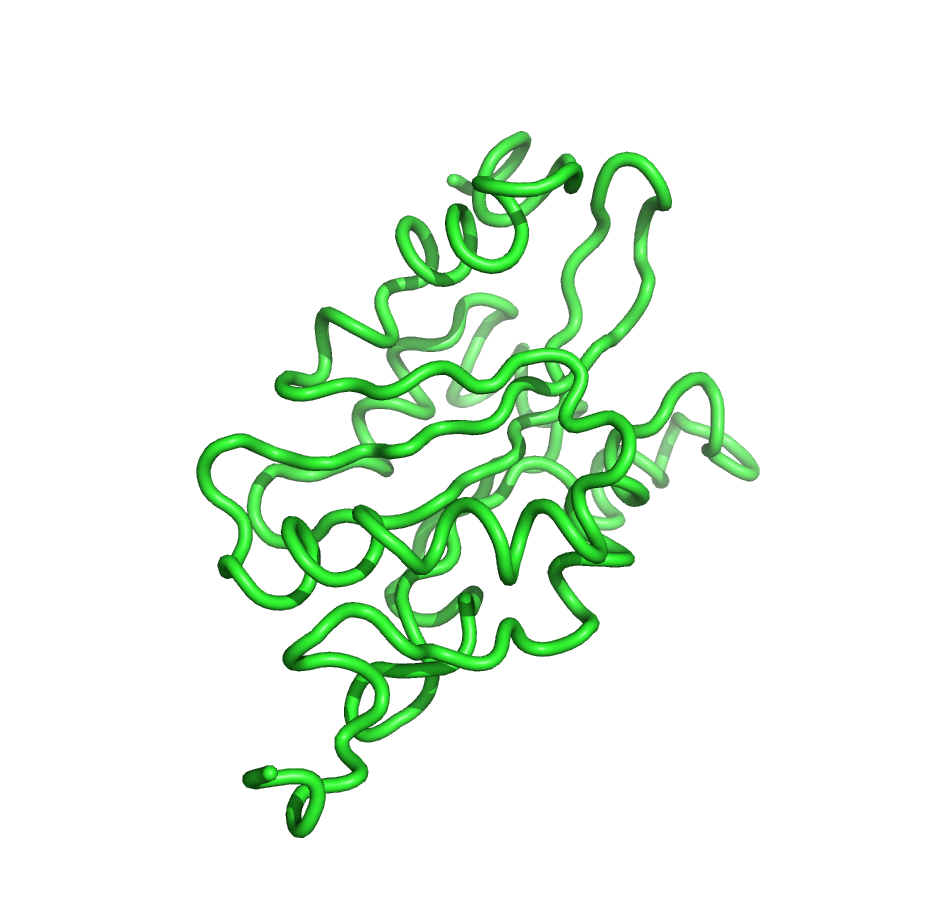
\includegraphics[width=\linewidth]{1ak6A00_true.png}
        \caption{True sample from CATH S40.}
        \label{fig:sample-true}
    \end{subfigure}
    \begin{subfigure}[b]{0.495\textwidth}
        \centering
        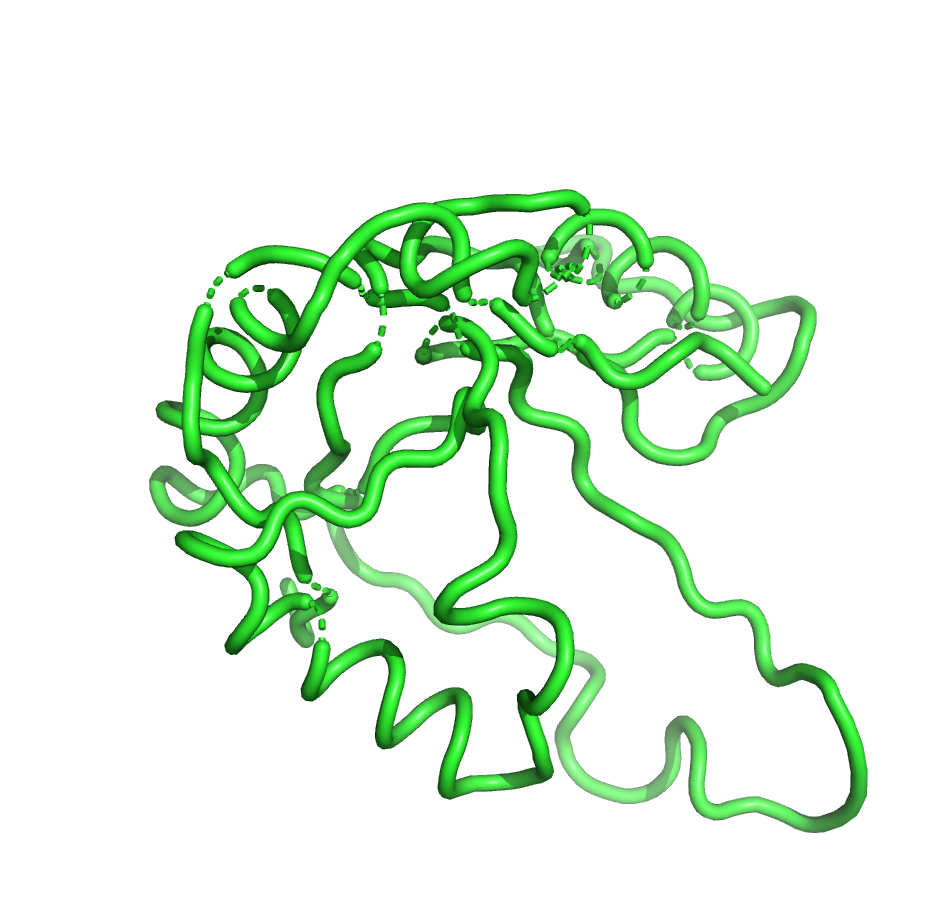
\includegraphics[width=0.95\linewidth]{1ak6A00_gen_unet.png}
        \caption{Sample from Unet model.}
        \label{fig:sample-unet}
    \end{subfigure}
    \begin{subfigure}[b]{0.495\textwidth}
        \centering
        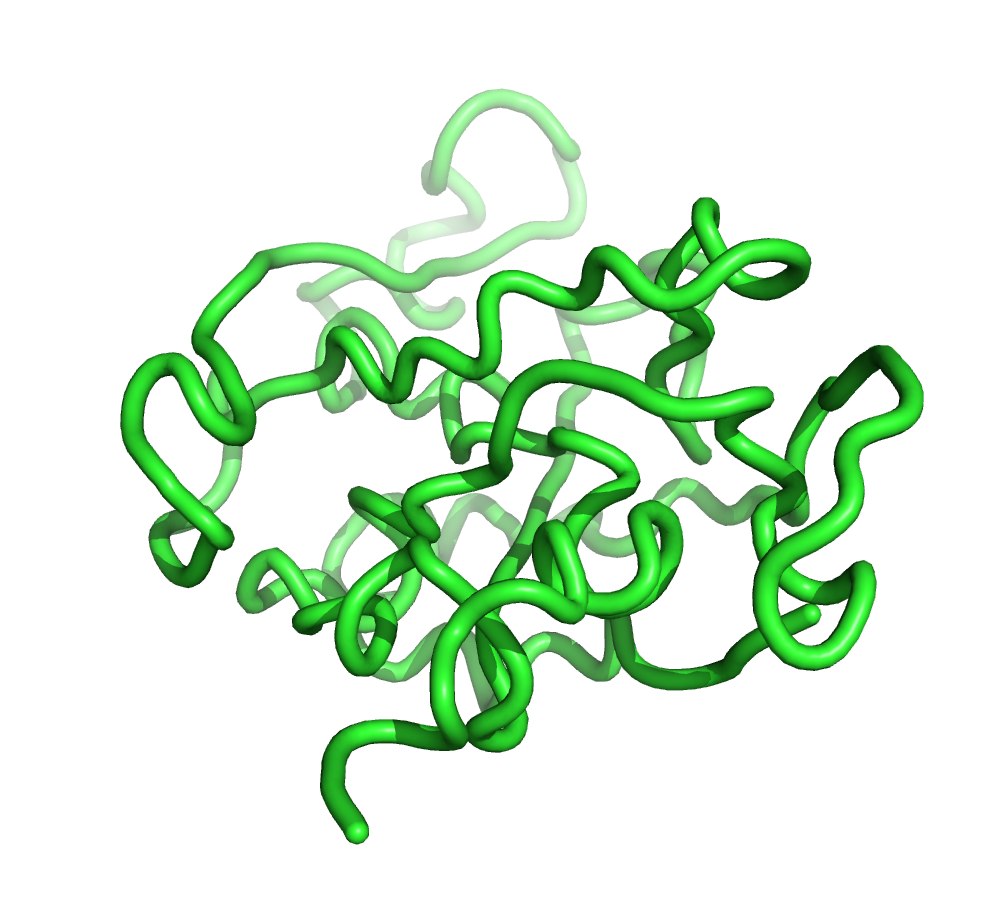
\includegraphics[width=\linewidth]{1ak6A00_gen_pos.png}
        \caption{Sample from GNN w/ positional encoding.}
        \label{fig:sample-pos}
    \end{subfigure}
    \begin{subfigure}[b]{0.48\textwidth}
        \centering
        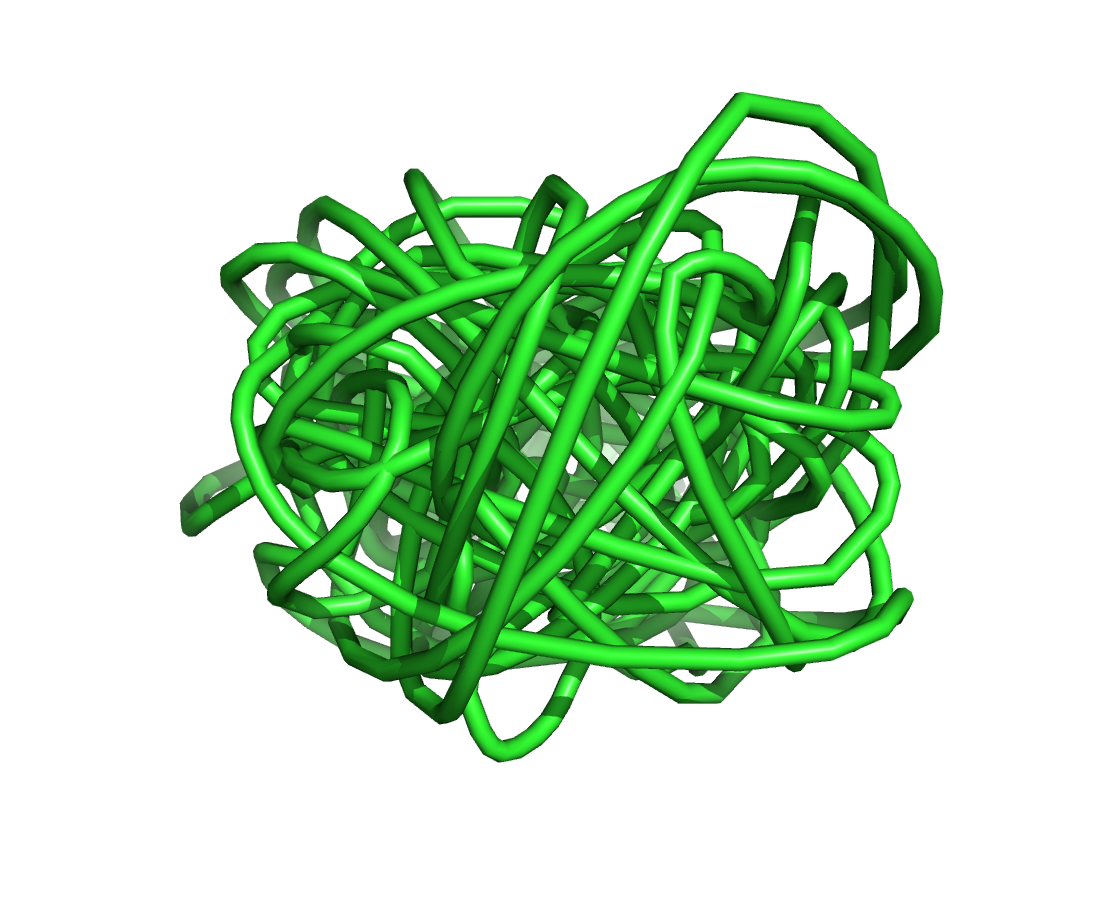
\includegraphics[width=\linewidth]{1a6fA00_gen_wo_pos.png}
        \caption{Sample from GNN w/o positional encoding.}
        \label{fig:sample-wo-pos}
    \end{subfigure}
    \caption{PyMOL visualisation of generated backbone samples from different models}
    \label{fig:samples}
\end{figure}

\subsection{Summary}\label{subsec:experiments-summary}
In summary, our experiments demonstrate that incorporating positional encodings into a Transformer-based graph convolutional network substantially improves backbone generation fidelity. Across quantitative metrics, the positional GCN achieved the lowest RMSD and highest TM-scores, outperforming both the UNet baseline and the GCN without positional information. Distributional analyses further showed that this model produces more consistent samples, while both quantitative results and qualitative visualisations highlighted that the absence of positional encodings often leads to collapsed or unrealistic folds.

At the same time, challenges remain. RMSD and TM-scores still indicate a gap between generated and native backbones, particularly for long chains where deviations accumulate. Individual qualitative examples provide intuition but do not fully capture the diversity of generated structures, suggesting the need for larger-scale structural assessments.

Overall, these results underscore the importance of combining geometric and sequential information when modelling proteins with diffusion processes. The following chapter discusses the broader implications of these findings, outlines limitations of the present work, and suggests directions for future research.

\clearpage

\section{Discussion and Conclusion}\label{sec:Discussion_and_Conclusion}
\subsection{Discussion of Results}\label{subsec:discussion-results}
The experiments in \cref{sec:Experiments} demonstrate that score-based diffusion models can generate protein backbones with meaningful structural similarity to native folds. Among the evaluated architectures, the Transformer-based GCN with positional embeddings consistently outperformed the UNet baseline and the GCN without positional encodings in both RMSD and TM-score. This finding underscores the importance of incorporating sequential order into graph-based architectures, complementing geometric edge features such as distances and orientations.

\subsection{Limitations}\label{subsec:limitations}
While the results are encouraging, several limitations must be acknowledged:
\begin{itemize}
    \item \textbf{Geometric constraints.} No explicit bond length or bond angle constraints were imposed during training or sampling. Although the model learns approximate geometry from data, explicit constraints would ensure chemical validity and prevent subtle violations of backbone stereochemistry \citep{branden2012IntroductionProteinStructure,creighton1993proteins,watsonNovoDesignProtein2023}.
    \item \textbf{Backbone-only representation.} Only C\(_\alpha\) atoms were modelled, ignoring side chains and residue types. This simplifies the state space but limits biological interpretability and applicability to sequence-conditioned design tasks.
    \item \textbf{Model scale.} The models used in this study are relatively small compared to state-of-the-art generative protein models \citep{wuProteinStructureGeneration2024,watsonNovoDesignProtein2023}. While we demonstrated feasibility even for backbones exceeding 1000 amino acids, scaling to larger networks with equivariant layers, global attention, or pretraining on larger structural databases may further improve results.
    \item \textbf{Evaluation metrics.} RMSD and TM-score measure fidelity to a specific native fold of length \(L\). However, a generated backbone with high RMSD or low TM may still correspond to a physically plausible alternative fold. Thus, our evaluation measures reconstruction fidelity rather than unconditional structural validity.
\end{itemize}

\subsection{Related Work and Future Directions}\label{subsec:future-work}
Recent years have seen rapid progress in generative modelling of protein structures. Diffusion-based methods in particular have achieved state-of-the-art results: \citet{watsonNovoDesignProtein2023} demonstrated that RoseTTAFold-based diffusion models can generate novel proteins with designed functions, while FoldingDiff \citep{wuProteinStructureGeneration2024} applied score-based diffusion directly to backbone coordinates. At the architectural level, SE(3)-equivariant neural networks \citep{satorras2021EquivariantGraphNeural,geiger2022E3nnEuclideanNeural} have been proposed to improve geometric fidelity and long-range modelling, building on earlier work in equivariant tensor field networks \citep{thomasTensorFieldNetworks2018,weiler3DSteerableCNNs2018,kondorClebschGordanNetsFully2018}. Inspired by these developments, as well as the limitations identified in this dissertation, several promising directions follow from this study.

\paragraph{Constraint integration.}
One natural extension is to incorporate stereochemical constraints directly into the generative process. In the present work, bond lengths, bond angles, and other relavant structural constraints were only learned approximately from data. Future models could embed these constraints within the diffusion dynamics, ensuring that generated samples lie on a physically valid manifold. Recent advances in Riemannian score-based generative modelling \citep{debortoliRiemannianScoreBasedGenerative2022,huang2022RiemannianDiffusionModels,chungImprovingDiffusionModels2022} provide a principled framework for defining diffusion processes and training objectives on constrained manifolds, which could be adapted to enforce protein backbone geometry explicitly. 

\paragraph{Advanced architectures.}
Another promising direction is to adopt architectures with built-in geometric equivariance. While the graph neural networks capture local geometry via edge features, it is not strictly equivariant under rotations or reflections. By contrast, SE(3)-equivariant GNNs \citep{thomasTensorFieldNetworks2018,weiler3DSteerableCNNs2018,kondorClebschGordanNetsFully2018,geiger2022E3nnEuclideanNeural,geiger2025EuclideanNeuralNetworks} encode these symmetries by construction, ensuring that predictions transform consistently with input coordinates. This property is particularly attractive for protein backbones, where physical laws are invariant to global orientation. Recent works \citep{yimDiffusionModelsProtein2024} have begun exploring this idea in the context of protein diffusion models.

\subsection{Conclusion}\label{subsec:conclusion}
This dissertation has explored the use of score-based diffusion models for protein backbone generation. We outlined the theoretical background of diffusion models, developed a graph-based representation of protein backbones, and implemented several neural architectures for score estimation. Experiments on the CATH S40 dataset showed that a residual Transformer-based GCN with positional embeddings achieved improved performance over both a UNet baseline and a graph model without positional information.

These results suggest that diffusion models combined with graph-based architectures offer a viable approach to coarse-grained protein structure generation. Although the models used here are relatively small in scale, the findings highlight the value of incorporating sequential information into graph representations and point toward directions for improvement, including constraint integration, larger architectures, and sequence conditioning.

\clearpage

\appendix
\section{Code Appendix}
% This appendix provides excerpts from the implementation of the graph neural network (GNN) model described in the main text (\cref{subsubsec:Transformer-GCN}). The code is written in Python and makes use of standard machine learning libraries, including PyTorch and PyTorch Geometric (PyG) \citep{PyG1.0,PyG2.0}. For readability, only the core components of the model are shown here. The complete source code used in this dissertation, including data preprocessing, training and sampling scripts, and relavant utilities, is available in the accompanying GitHub repository: \url{TODO}. %TODO: link here
% \begin{minted}[linenos,breaklines,breaksymbolleft={},breaksymbolright={},frame=single,framesep=2mm,baselinestretch=1.05,]{python}
% class GraphTransformerScoreModel(nn.Module):
%     def __init__(self, hidden_dim=128, pos_embed_dim=128, t_embed_dim=128, t_edge_proj_dim=16, num_layers=5, heads=8, max_num_neighbors=500, radius=5, num_basis=32):
%         super().__init__()
%         self.max_num_neighbors = max_num_neighbors
%         self.radius = radius
%         self.num_basis = num_basis
%         self.heads = heads

%         # position embedding
%         self.pos_embed = nn.Sequential(
%             SinusoidalEncoding(embed_dim=pos_embed_dim),
%             nn.Linear(pos_embed_dim, pos_embed_dim)
%         )

%         # position MLPs per layer
%         self.pos_mlps = nn.ModuleList([
%             nn.Linear(pos_embed_dim, pos_embed_dim) for _ in range(num_layers)
%         ])

%         # Time embedding
%         self.t_embed = nn.Sequential(
%             GaussianFourierProjection(t_embed_dim, scale=16.),
%             nn.Linear(t_embed_dim, t_embed_dim),
%         )

%         self.t_edge_proj = nn.Linear(t_embed_dim, t_edge_proj_dim)

%         # Time MLPs per layer
%         self.t_mlps = nn.ModuleList([
%             nn.Linear(t_embed_dim, t_embed_dim) for _ in range(num_layers)
%         ])

%         # TransformerConv layers
%         in_channels = hidden_dim + pos_embed_dim + t_embed_dim
%         self.convs = nn.ModuleList([
%             TransformerConv(
%                 in_channels=in_channels,
%                 out_channels=hidden_dim // heads,
%                 heads=heads,
%                 concat=True,
%                 beta=True,
%                 edge_dim=self.num_basis + 3 + t_edge_proj_dim
%             )
%             for _ in range(num_layers)
%         ])

%         # Norm layers
%         self.norms = nn.ModuleList([
%             GraphNorm(hidden_dim) for _ in range(num_layers)
%         ])

%         # Input/output projection
%         self.input_proj = nn.Linear(3, hidden_dim)
%         self.output_proj = nn.Sequential(
%             nn.Linear(hidden_dim, hidden_dim),
%             nn.SiLU(),
%             nn.Linear(hidden_dim, 3)
%         )

%         self.act = nn.SiLU()

%     def forward(self, coords, batch, t):
%         # Positional encoding (based on position index in the chain)
%         num_graphs = batch.max().item() + 1
%         pos_index = torch.empty_like(batch, dtype=torch.float)
%         for i in range(num_graphs):
%             mask = (batch == i)
%             count = mask.sum()
%             pos_index[mask] = torch.linspace(0, 1, steps=count, device=coords.device)
%         pos_feat = self.act(self.pos_embed(pos_index[:, None]))  # [N, pos_embed_dim]

%         # Time embedding
%         t_feat = self.act(self.t_embed(t[:, None]))  # [B, t_embed_dim]

%         # Node features
%         h = self.input_proj(coords)  # [N, hidden_dim]

%         # Build radius graph to get the edge index
%         edge_index = radius_graph(coords, r=self.radius, batch=batch, max_num_neighbors=self.max_num_neighbors, loop=True, flow='target_to_source')

%         # edge attributes
%         edge_vec = coords[edge_index[0]] - coords[edge_index[1]]
%         edge_dir = F.normalize(edge_vec, dim=-1)
%         edge_length = edge_vec.norm(dim=-1)
%         edge_scalar = soft_one_hot_linspace(
%             edge_length,
%             start=0.0,
%             end=self.radius,
%             number=self.num_basis,
%             basis='gaussian',
%             cutoff=True
%         )  # [num_edges, num_basis]
%         t_edge = t_feat[batch][edge_index[0]]   # [num_edges, t_embed_dim]
%         t_edge = self.t_edge_proj(t_edge)   # [num_edges, t_edge_proj_dim]
%         # Combine with direction vectors
%         edge_attr = torch.cat([edge_scalar, edge_dir, t_edge], dim=-1)  # [num_edges, num_basis + 3 + t_edge_proj_dim]

%         for conv, norm, pos_mlp, t_mlp in zip(self.convs, self.norms, self.pos_mlps, self.t_mlps):
%             t_per_node = t_mlp(t_feat)[batch]  # [N, t_embed_dim]
%             pos = pos_mlp(pos_feat)

%             # Residual
%             h_res = h

%             # Concat time + feature
%             h = conv(torch.cat([h, pos, t_per_node], dim=-1), edge_index=edge_index, edge_attr=edge_attr)

%             # Normalization + residual
%             h = self.act(norm(h, batch) + h_res)

%         return self.output_proj(h)


% class SinusoidalEncoding(nn.Module):
%     def __init__(self, embed_dim=128):
%         super().__init__()
%         self.embed_dim = embed_dim

%     def forward(self, pos_index):
%         i = torch.arange(self.embed_dim, device=pos_index.device)
%         angle_rates = 1 / torch.pow(10000, (2 * (i // 2)) / self.embed_dim)
%         angle_rads = pos_index * angle_rates
%         angle_rads[:, 0::2] = torch.sin(angle_rads[:, 0::2])
%         angle_rads[:, 1::2] = torch.cos(angle_rads[:, 1::2])
%         return angle_rads


% class GaussianFourierProjection(nn.Module):
%     def __init__(self, embed_dim, scale=30.):   # embed_dim must be divisible by 2
%         super().__init__()
%         self.W = nn.Parameter(torch.randn(embed_dim // 2) * scale, requires_grad=False)

%     def forward(self, t):
%         x_proj = 2 * torch.pi * t * self.W  # [B, D/2]
%         return torch.cat([torch.sin(x_proj), torch.cos(x_proj)], dim=-1)
% \end{minted}

\clearpage

\bibliographystyle{apalike}
\bibliography{references}
\end{document}
